\chapter{\texorpdfstring{\acs{DTC}}{DTC} scans over $\gamma$ and $K$}
\label{app:DTC-scans}

As introduced in Sec. \ref{subsec:train-test-DTC}, this Appendix summarises the reconstruction ability of the \ac{TAE} and the evolution of $L_\text{TAE}$ and $L_\text{TSC}$ through epochs of the training performed to determine the appropriate value of $\gamma$ weighting the two losses and the number of clusters $K$ to be considered in the \textit{train} phase of the \ac{DTC}. The results are reported separately for the two detectors, V08682A and V08682B.

%=====================================================================
\section{V08682A}
\label{app:DTC-scans-A}
%=====================================================================

\subsection{\texorpdfstring{$\bm{\gamma}$}{gamma} scan results}
Figures \ref{fig:scan-reconstruction_and_losses-gamma10}, \ref{fig:scan-reconstruction_and_losses-gamma100}, \ref{fig:scan-reconstruction_and_losses-gamma1000} and \ref{fig:scan-reconstruction_and_losses-gamma10000} show the reconstruction ability and the losses trend for $\gamma= 10, 100, 1000$ and $10000$ respectively.

Beyond the points discussed in the main text, the extremes highlight a clear trade-off: with $\gamma = 10$, the losses flatline and the clustering simply does not kick in, while at $\gamma = 10000$, the clustering loss does go down, but heavily penalizes reconstruction, making it the worst among all tested configurations. That leaves $\gamma = 1000$ as the sweet spot, being the only setting where both losses steadily decrease together across epochs while keeping assignments stable, with fewer than 15\% of events shifting clusters after epoch 3.

\begin{figure}[H]
    \centering
    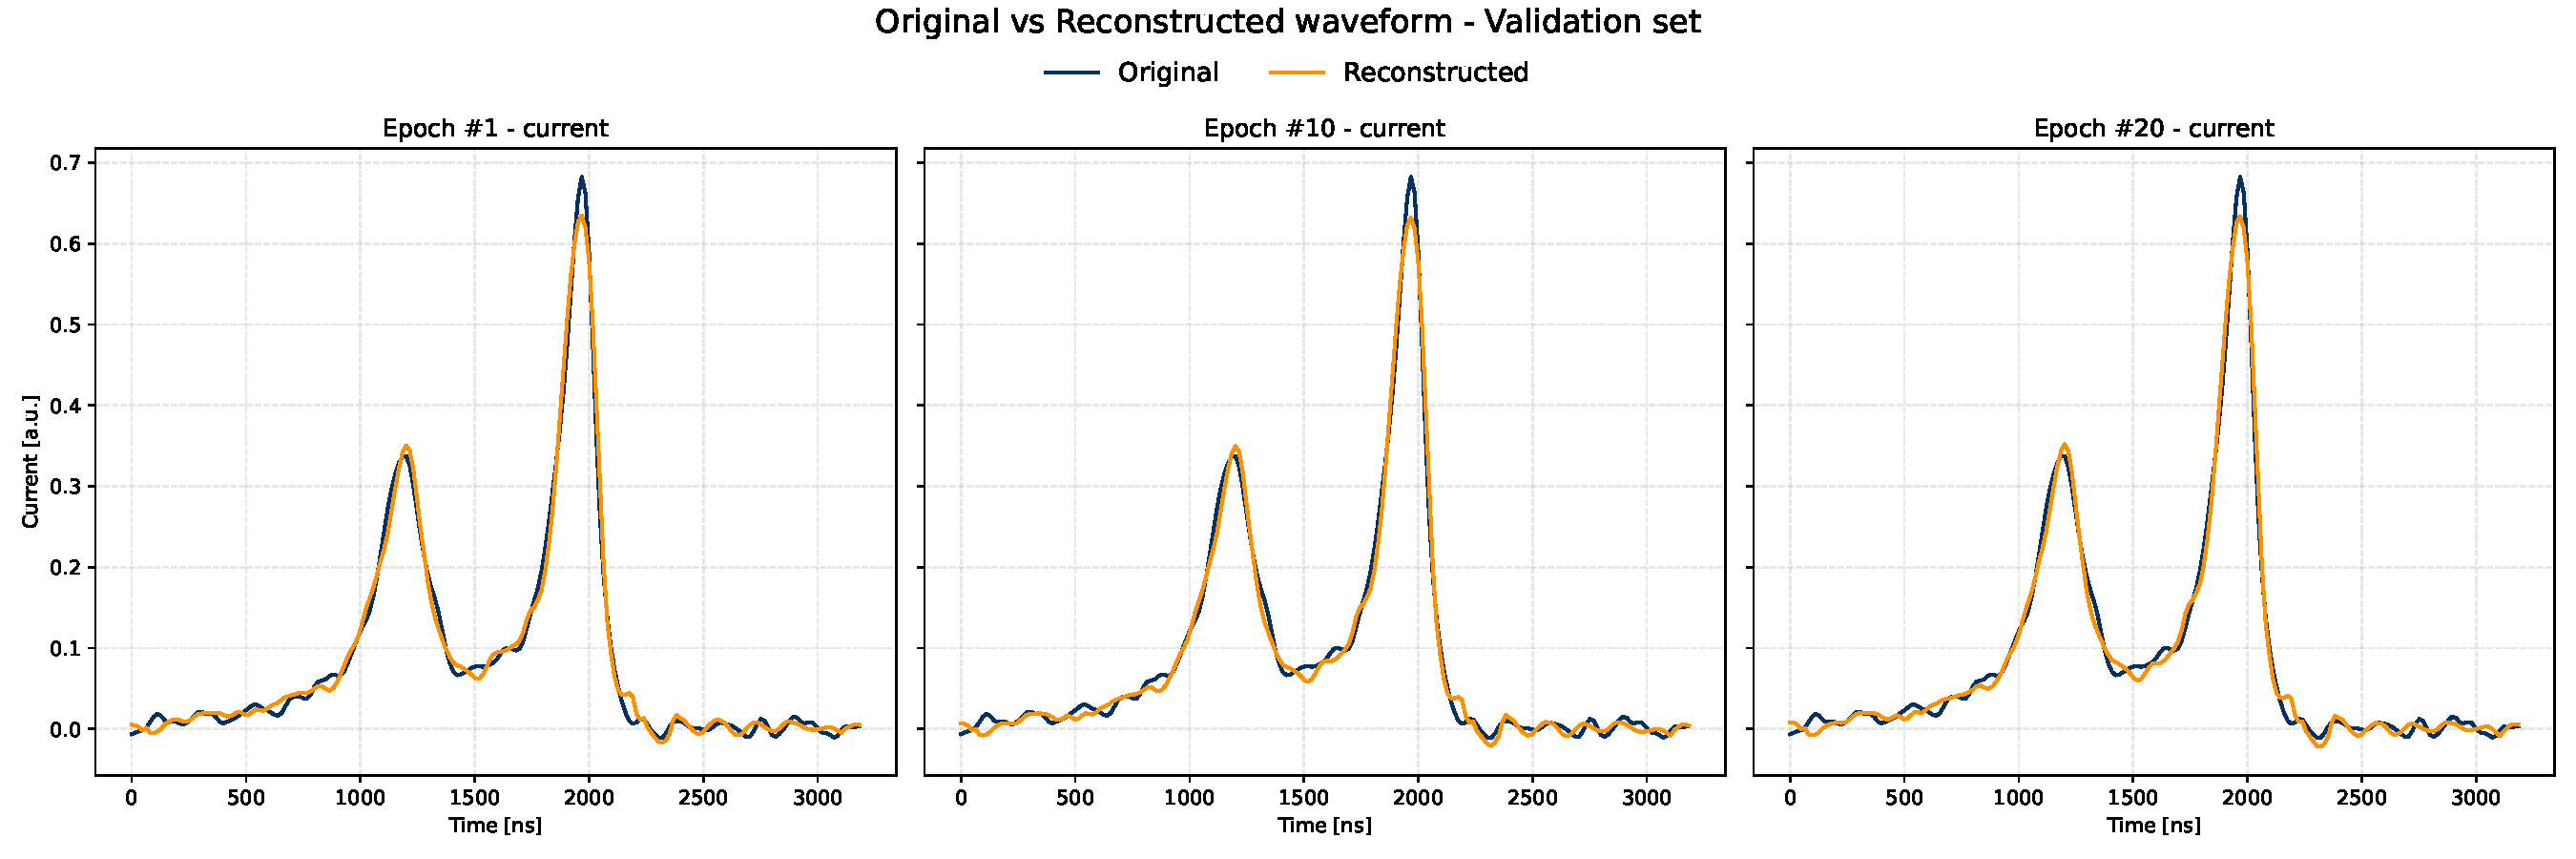
\includegraphics[width=\textwidth]{plots/DTC/gamma_scan/scan_eucl_gamma10_2cl_training_reconstruction.pdf}
    \par\medskip
    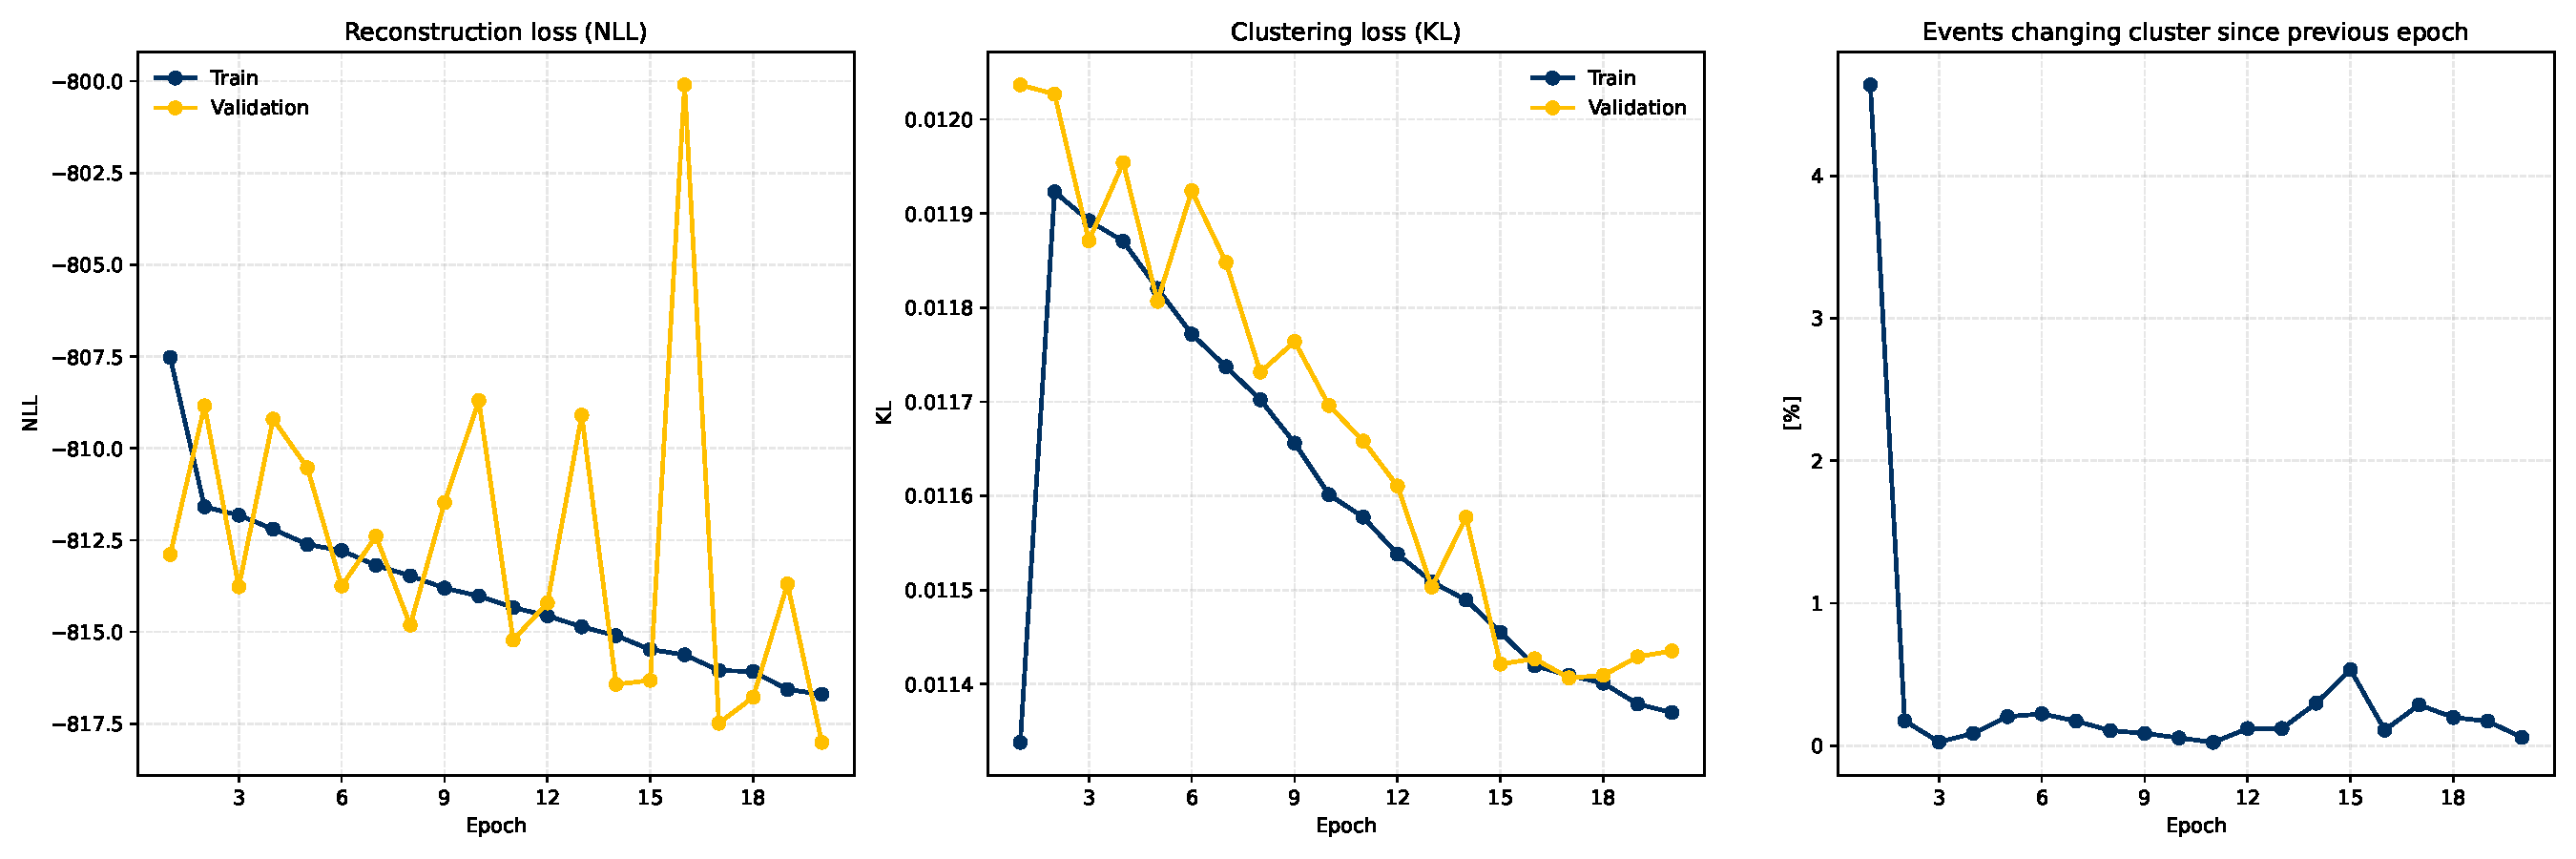
\includegraphics[width=\textwidth]{plots/DTC/gamma_scan/scan_eucl_gamma10_2cl_training_history.pdf}
    \caption{Training reconstruction and training losses for $\gamma=10$ with Euclidean Distance metric (V08682A).}
    \label{fig:scan-reconstruction_and_losses-gamma10}
\end{figure}

\begin{figure}[H]
    \centering
    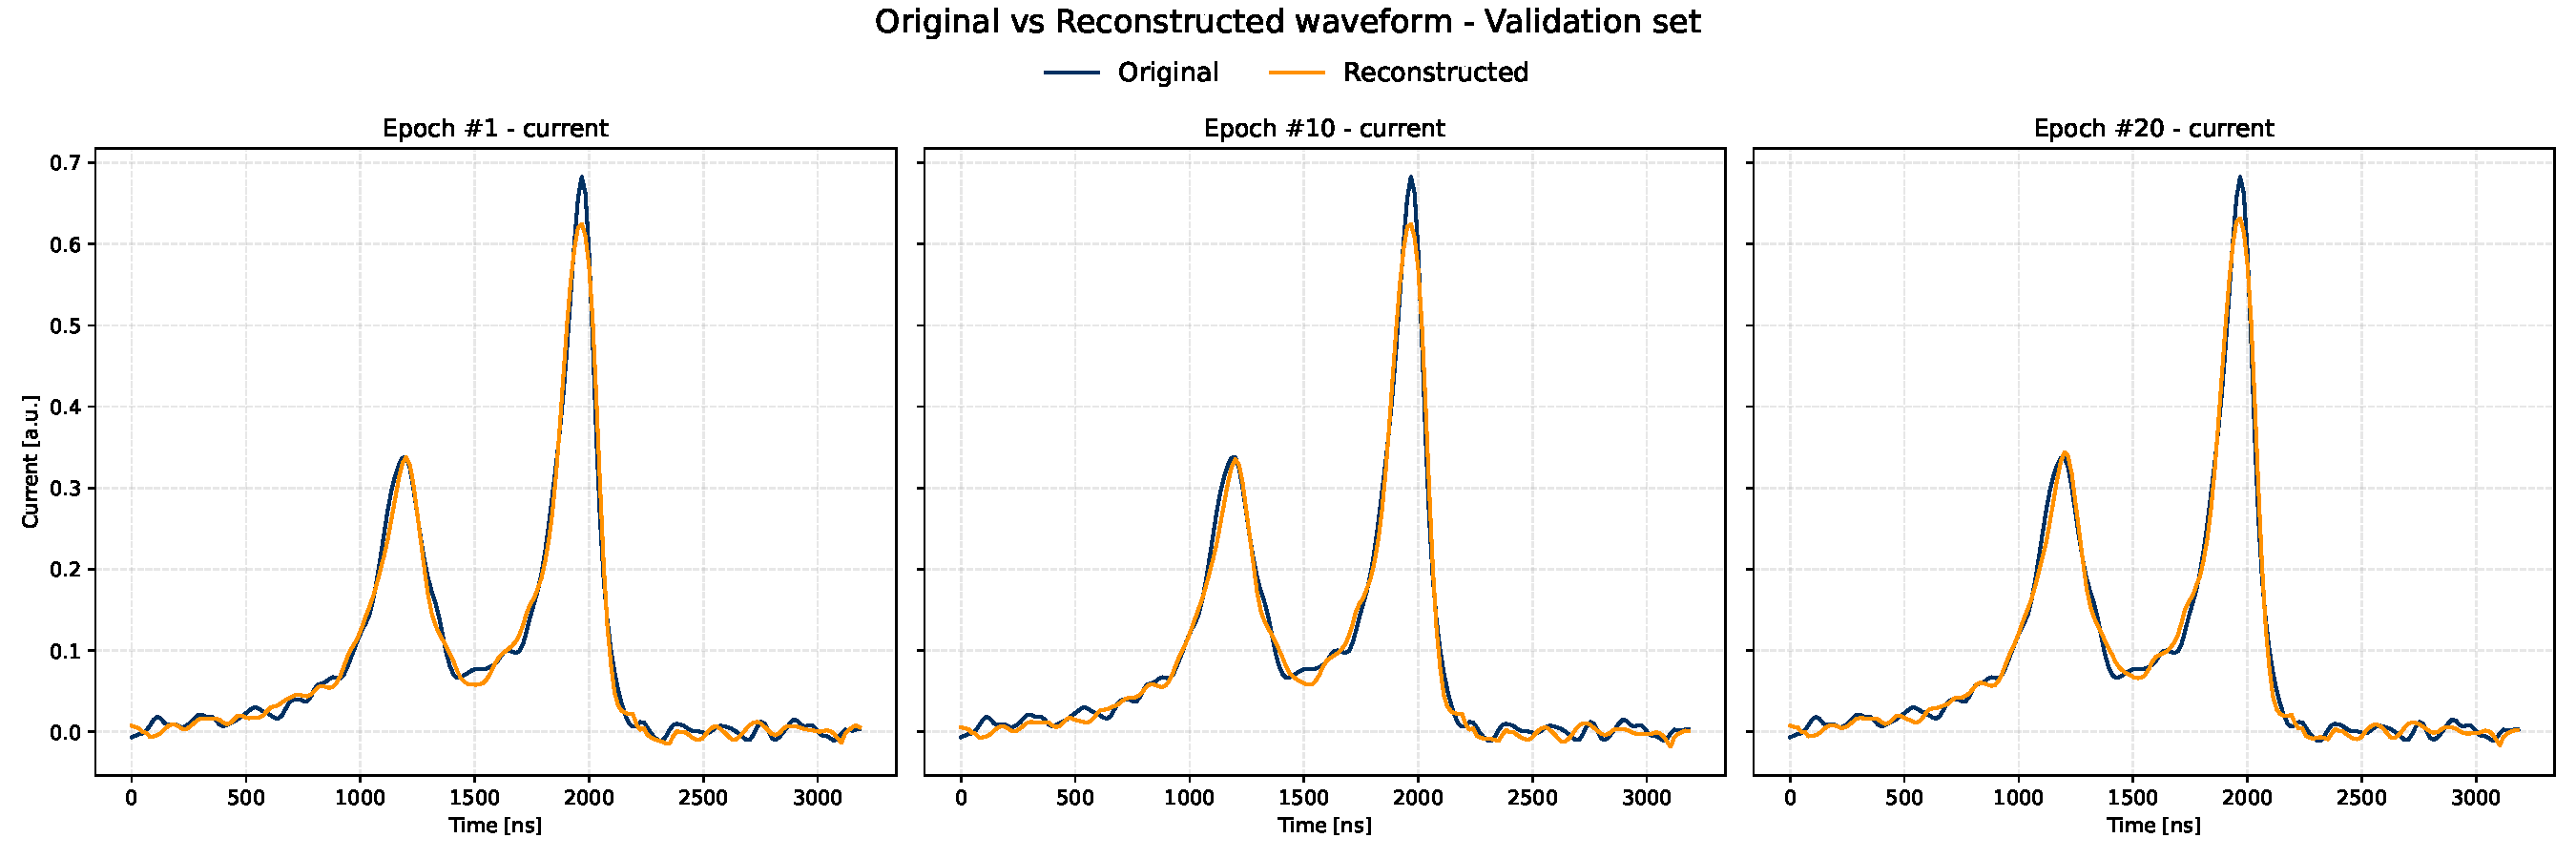
\includegraphics[width=\textwidth]{plots/DTC/gamma_scan/scan_eucl_gamma100_2cl_training_reconstruction.pdf}
    \par\medskip
    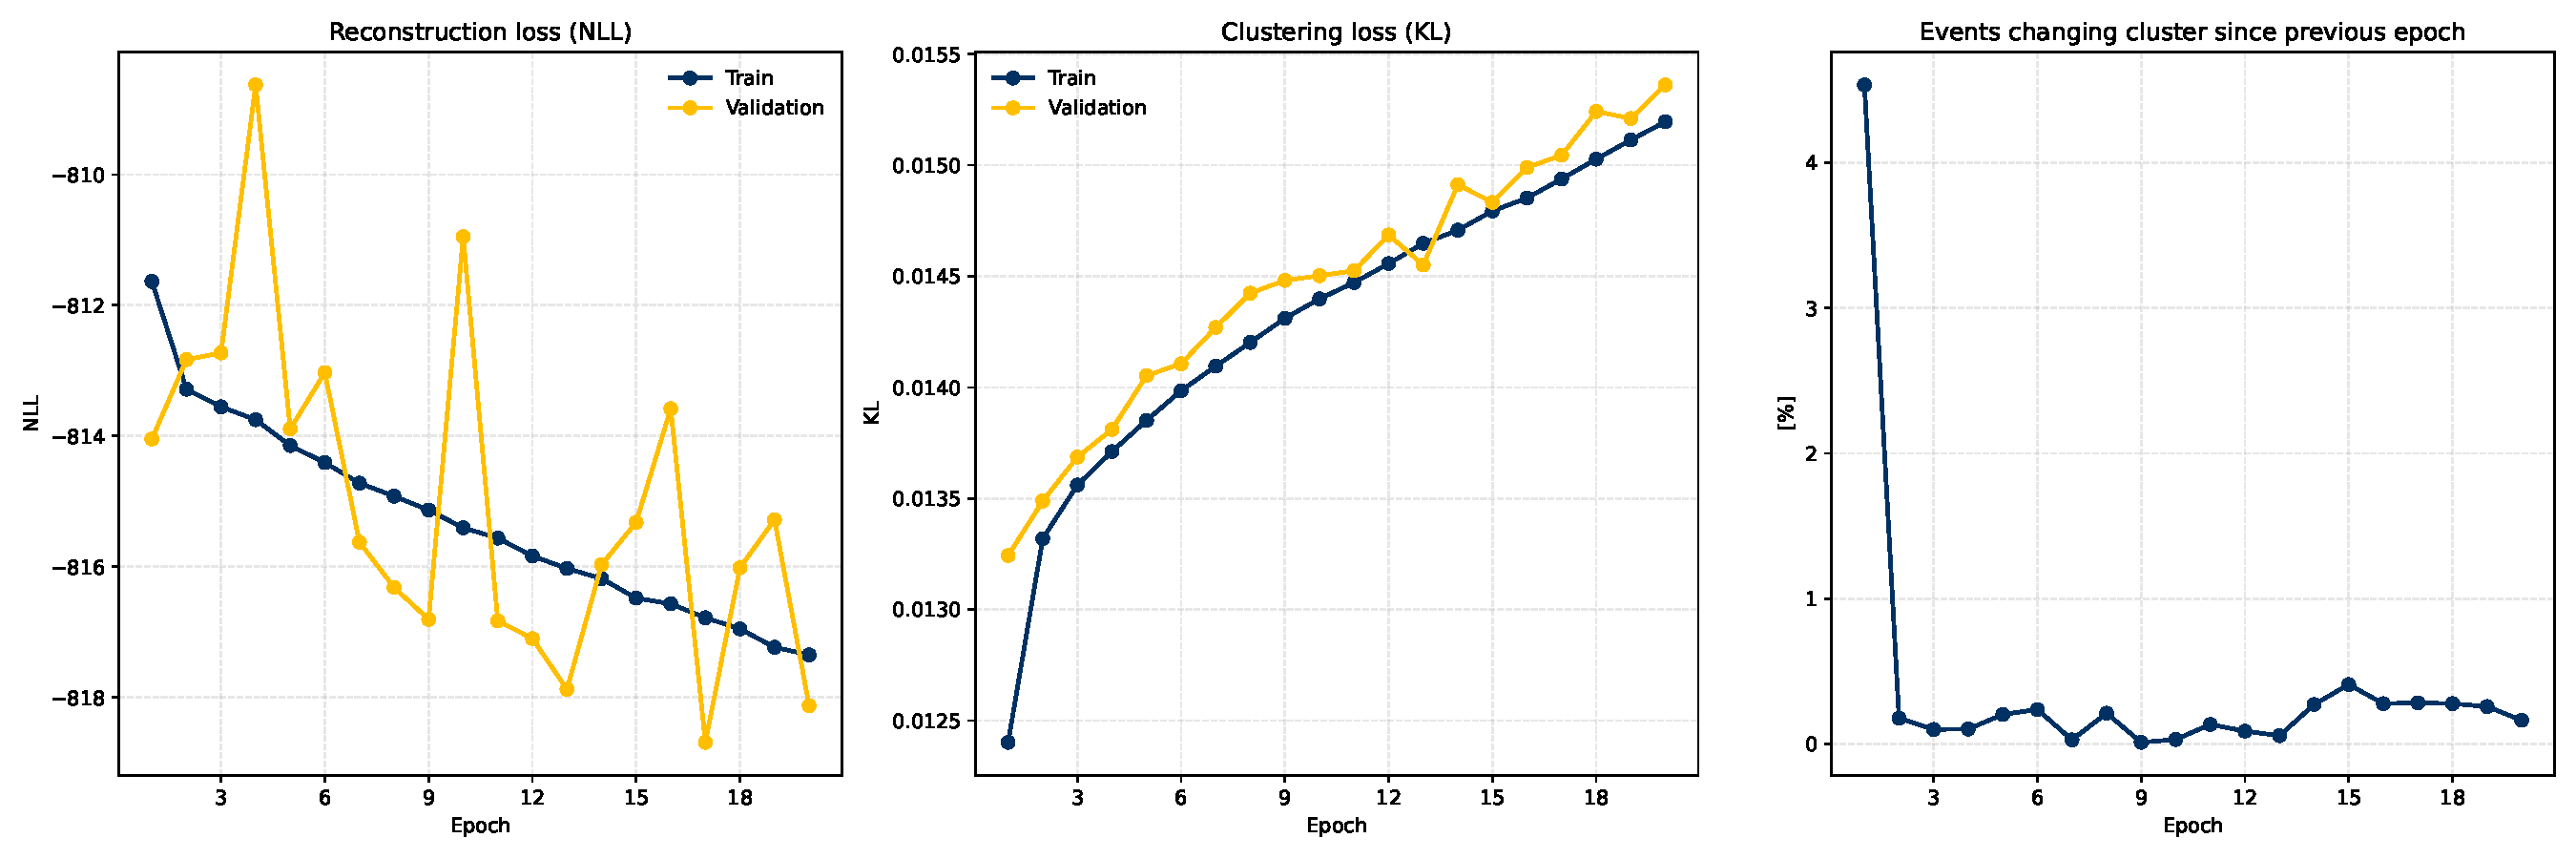
\includegraphics[width=\textwidth]{plots/DTC/gamma_scan/scan_eucl_gamma100_2cl_training_history.pdf}
    \caption{Training reconstruction and training losses for $\gamma=100$ with Euclidean Distance metric (V08682A).}
    \label{fig:scan-reconstruction_and_losses-gamma100}
\end{figure}

\begin{figure}[H]
    \centering
    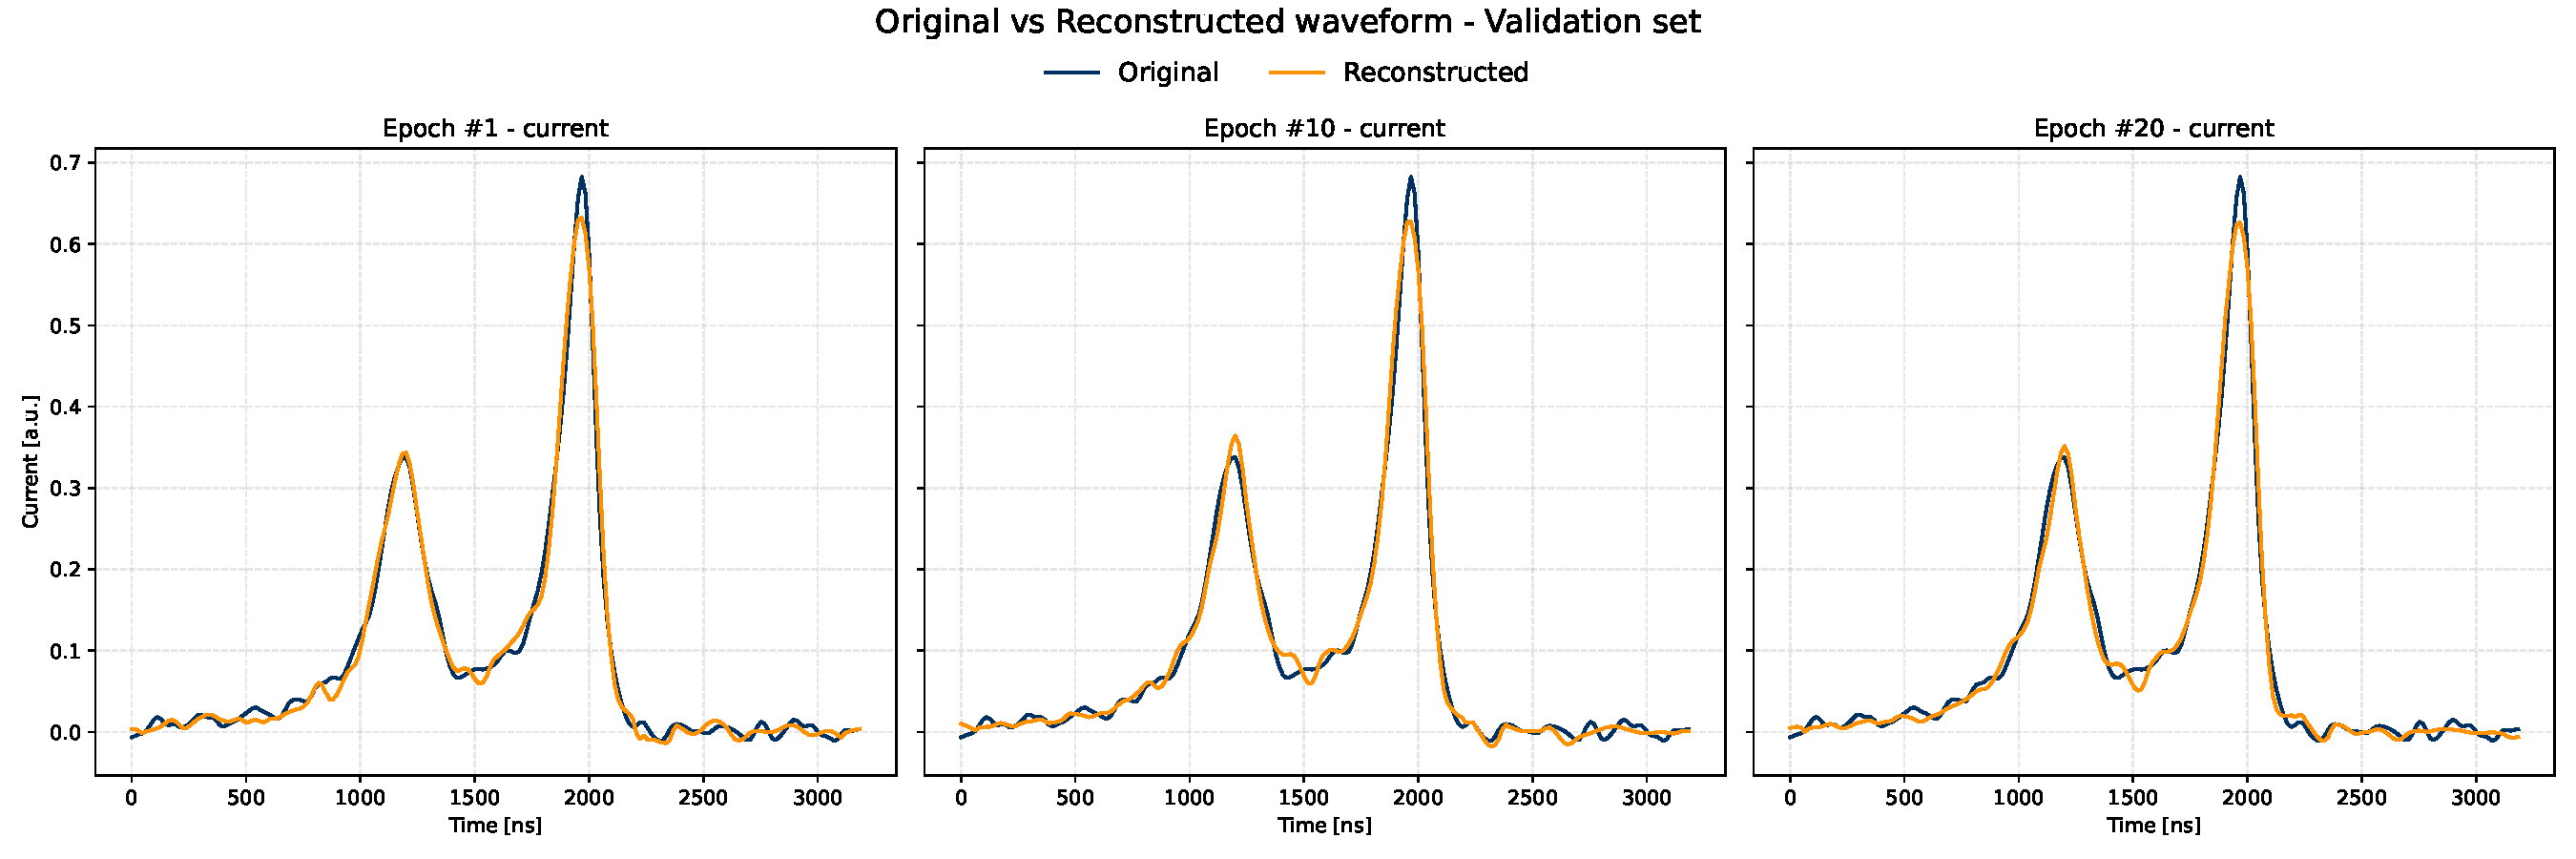
\includegraphics[width=\textwidth]{plots/DTC/gamma_scan/scan_eucl_gamma1000_2cl_training_reconstruction.pdf}
    \par\medskip
    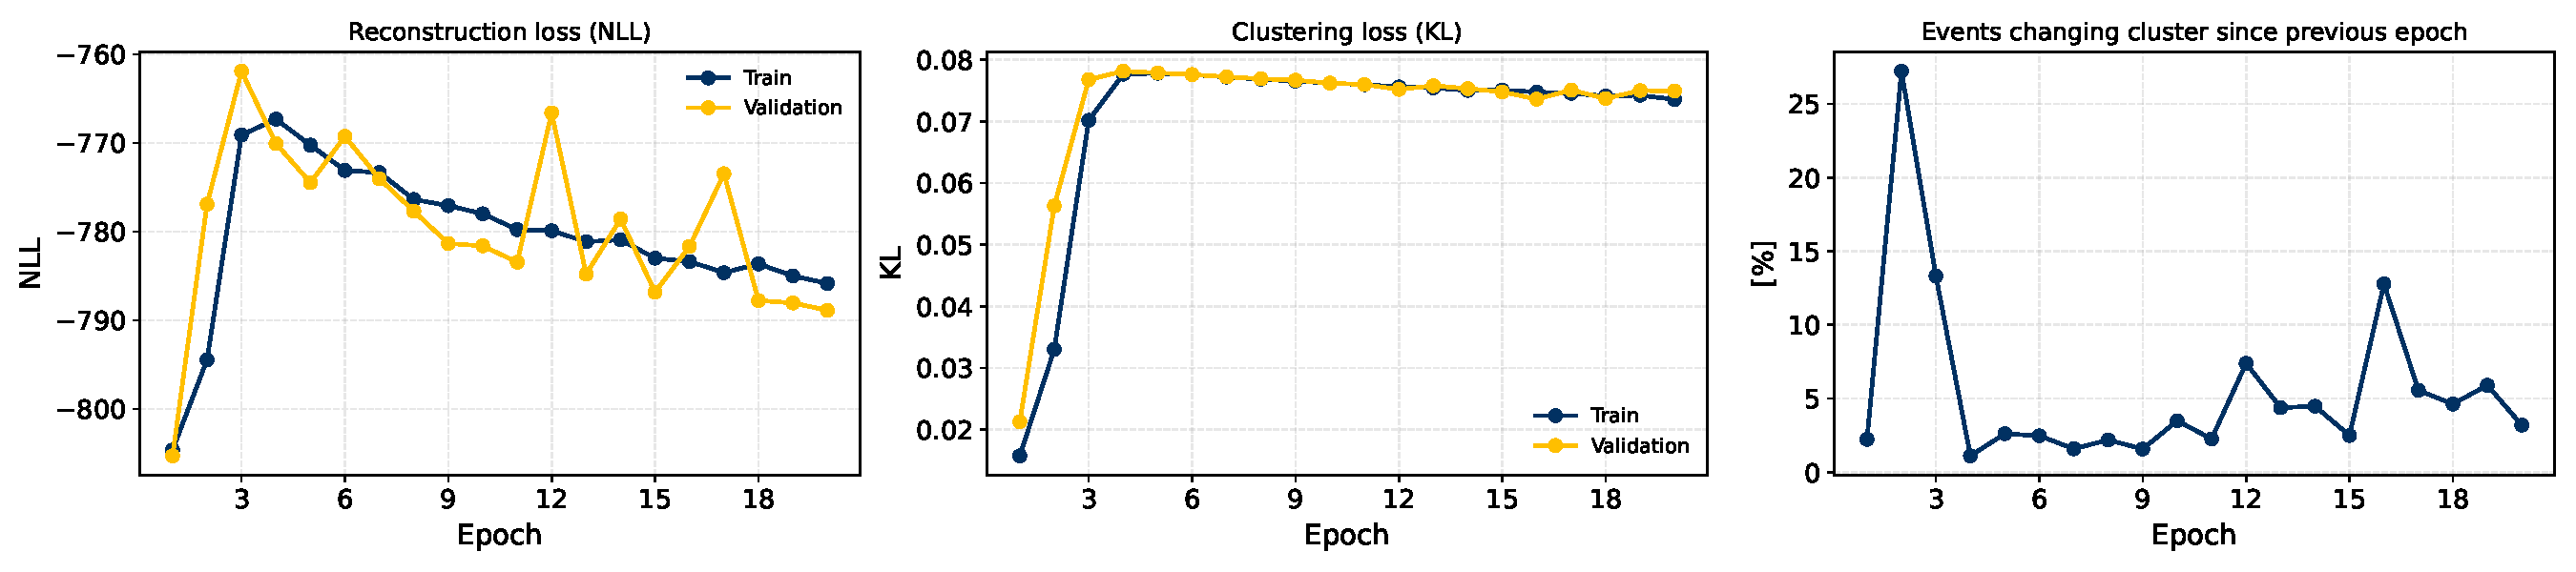
\includegraphics[width=\textwidth]{plots/DTC/gamma_scan/scan_eucl_gamma1000_2cl_training_history.pdf}
    \caption{Training reconstruction and training losses for $\gamma=1000$ with Euclidean Distance metric (V08682A).}
    \label{fig:scan-reconstruction_and_losses-gamma1000}
\end{figure}

\begin{figure}[H]
    \centering
    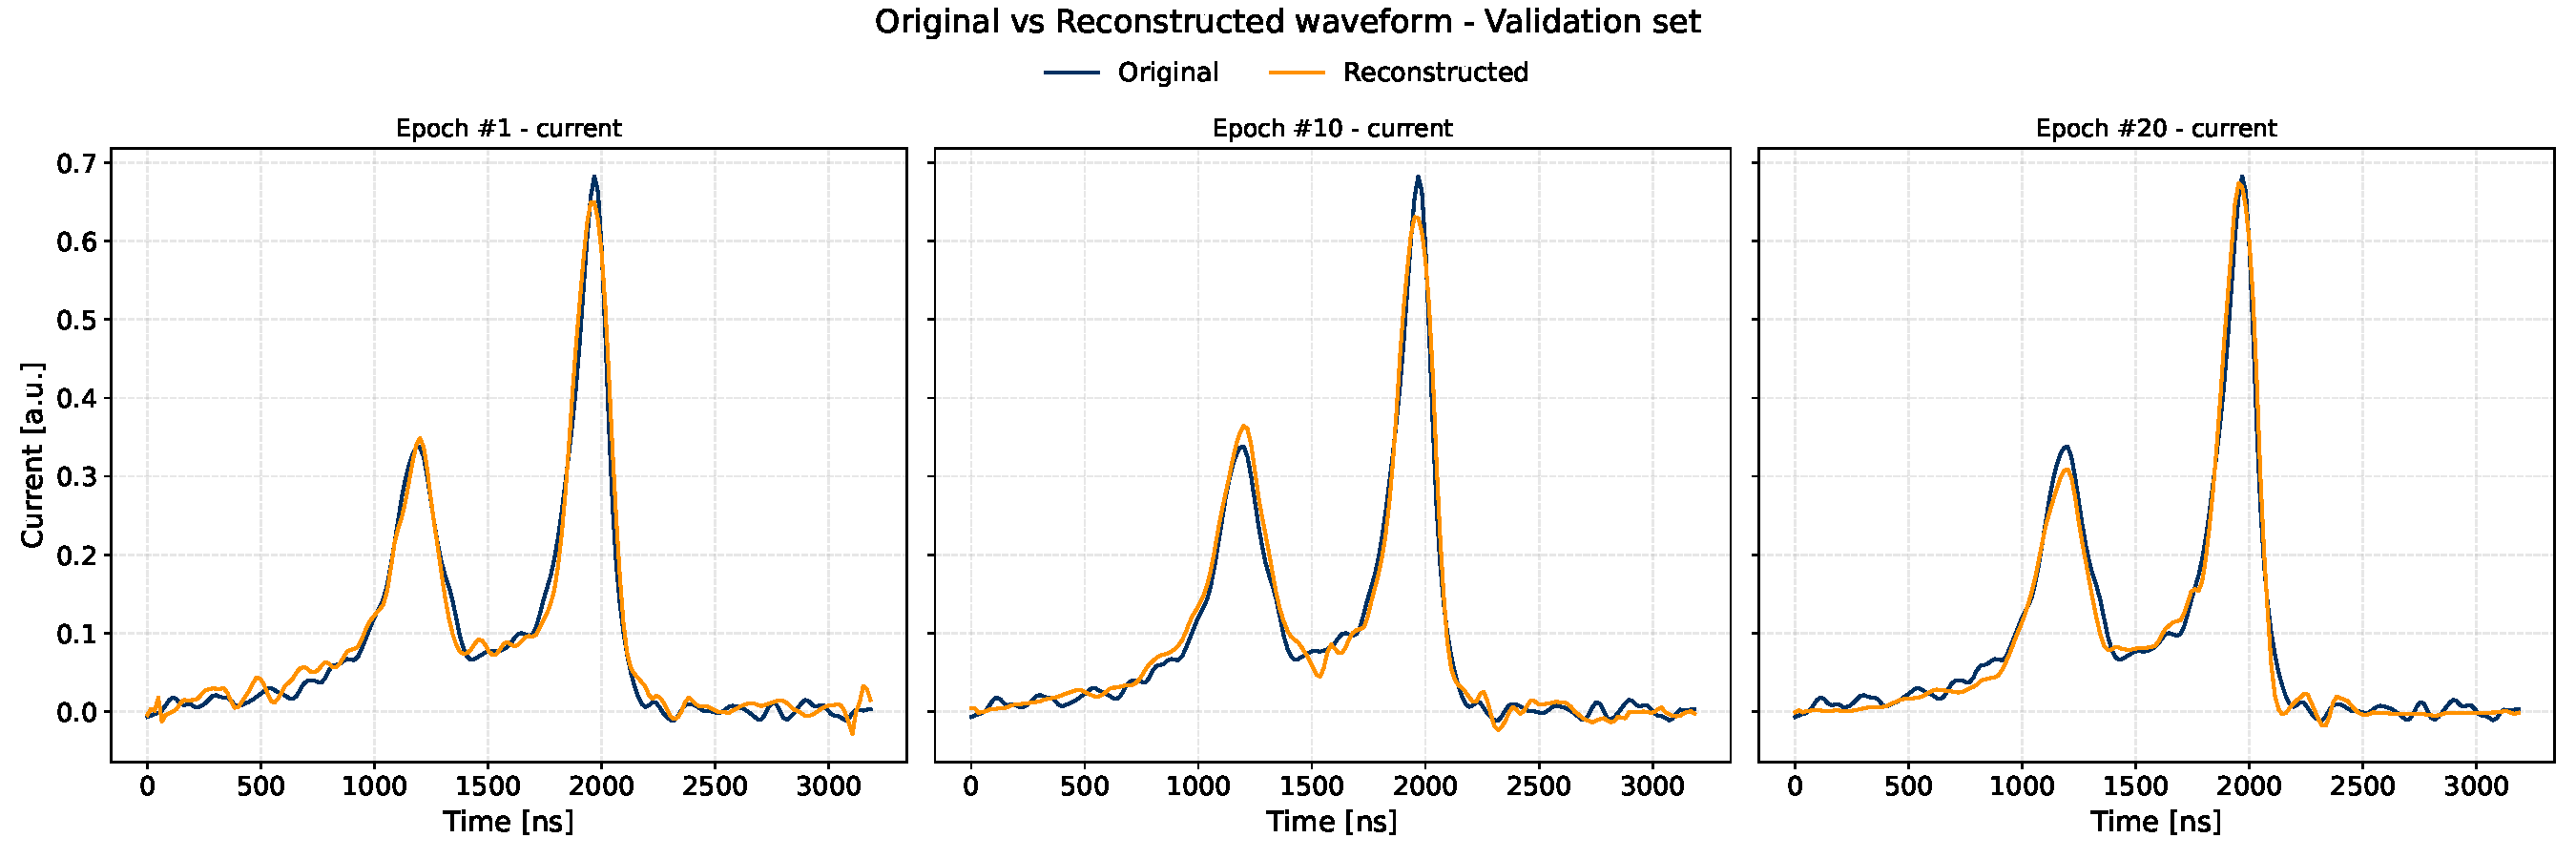
\includegraphics[width=\textwidth]{plots/DTC/gamma_scan/scan_eucl_gamma10000_2cl_training_reconstruction.pdf}
    \par\medskip
    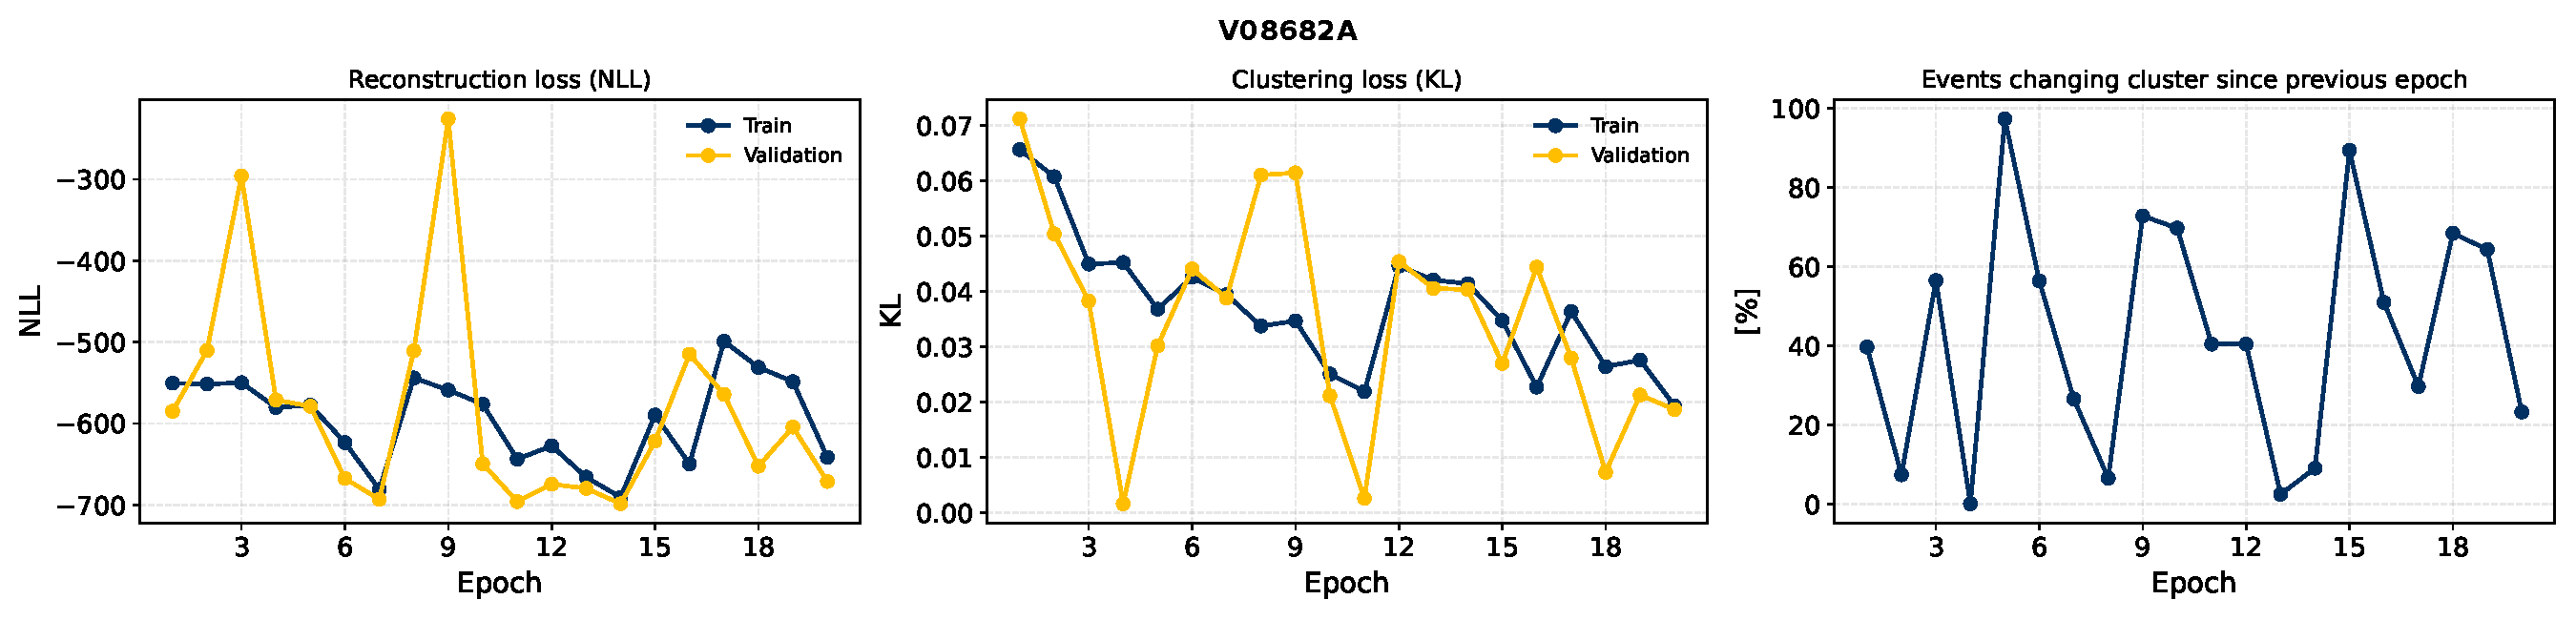
\includegraphics[width=\textwidth]{plots/DTC/gamma_scan/scan_eucl_gamma10000_2cl_training_history.pdf}
    \caption{Training reconstruction and training losses for $\gamma=10000$ with Euclidean Distance metric (V08682A).}
    \label{fig:scan-reconstruction_and_losses-gamma10000}
\end{figure}

\subsection{Clusters scan results}
As introduced in Sec. \ref{subsec:train-test-DTC}, Figures \ref{fig:scan-reconstruction_and_losses-K3} and \ref{fig:scan-reconstruction_and_losses-K4} show the reconstruction ability and the losses trend for $K= 3$ and $4$ respectively, where $K$ is the number of clusters. The $K=2$ configuration is not reported here since it is precisely the one of Fig. \ref{fig:scan-reconstruction_and_losses-gamma1000} of the previous Subsection.

\begin{figure}[H]
    \centering
    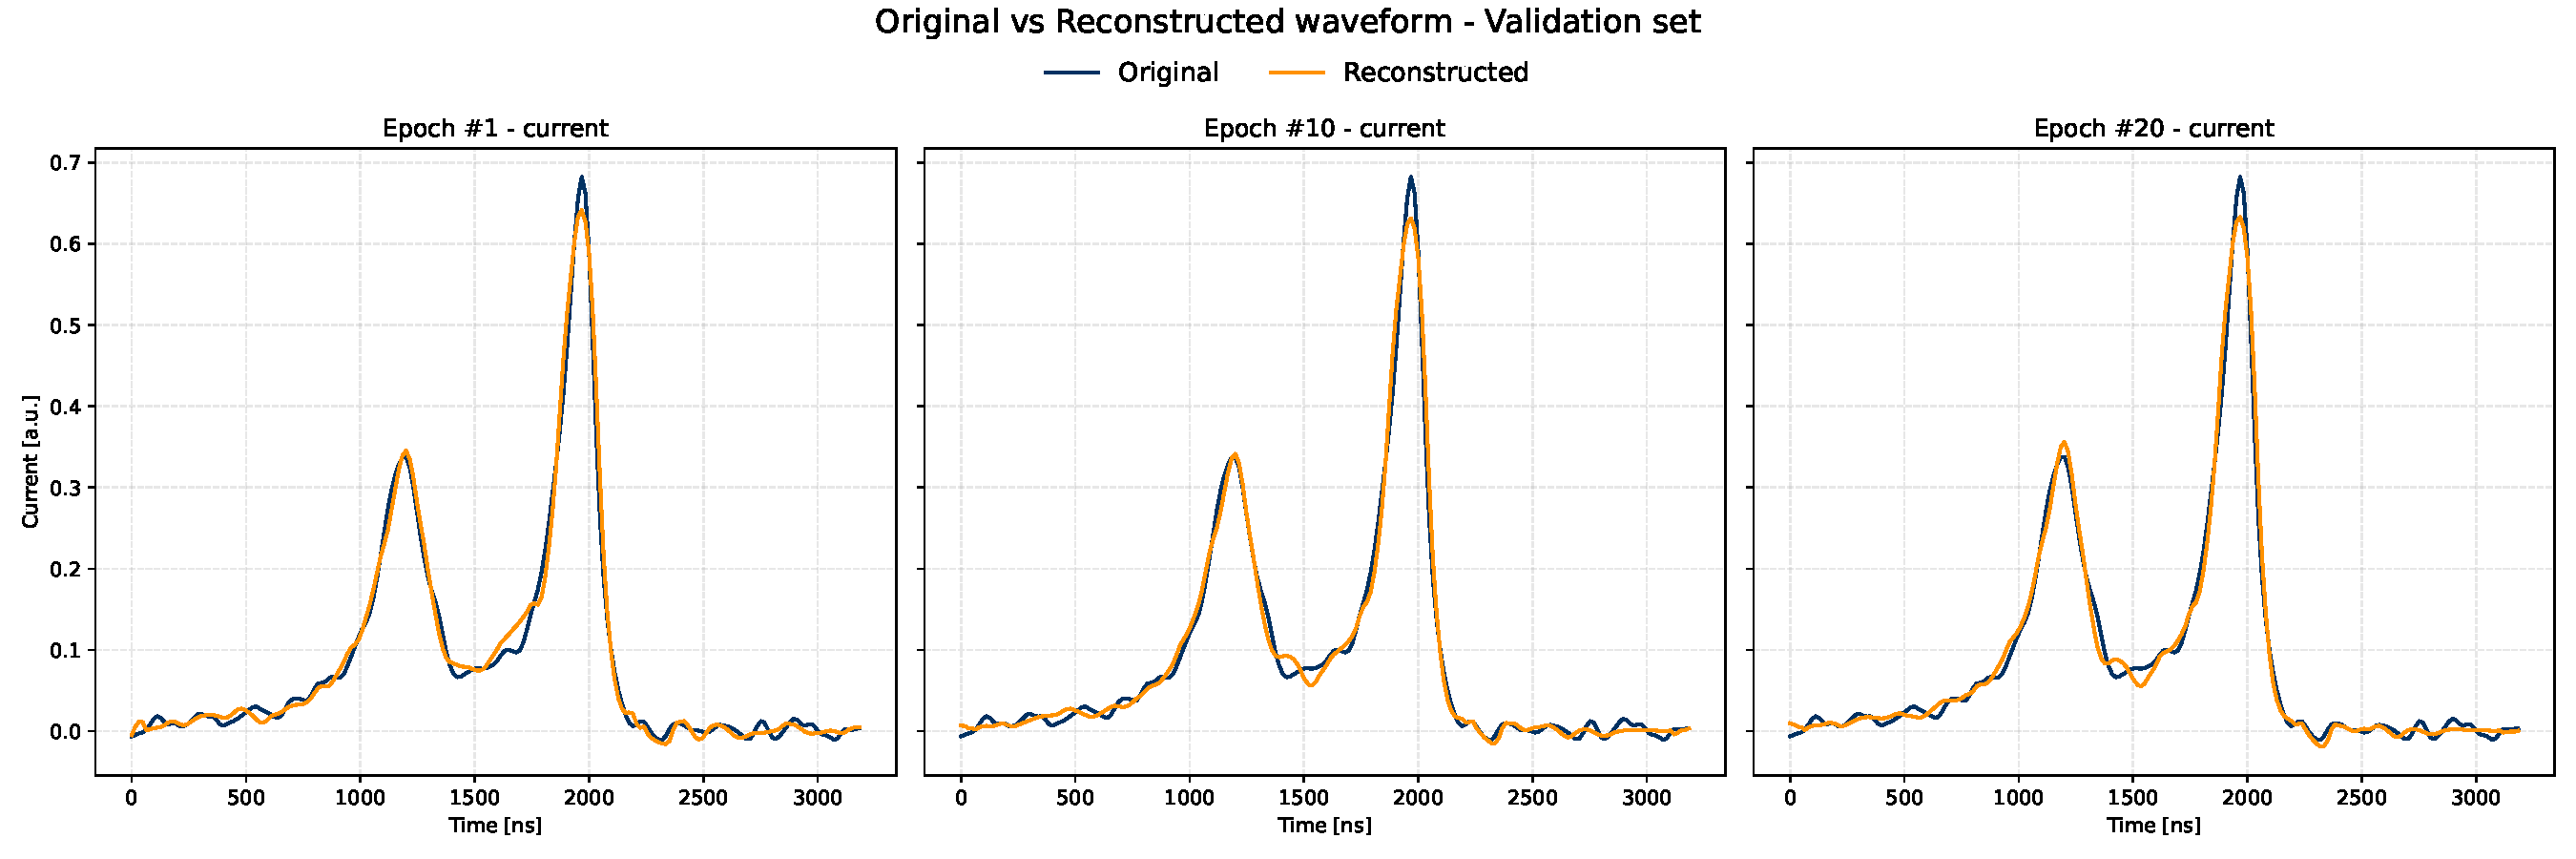
\includegraphics[width=\textwidth]{plots/DTC/clusters_scan/scan_eucl_3cl_training_reconstruction.pdf}
    \par\medskip
    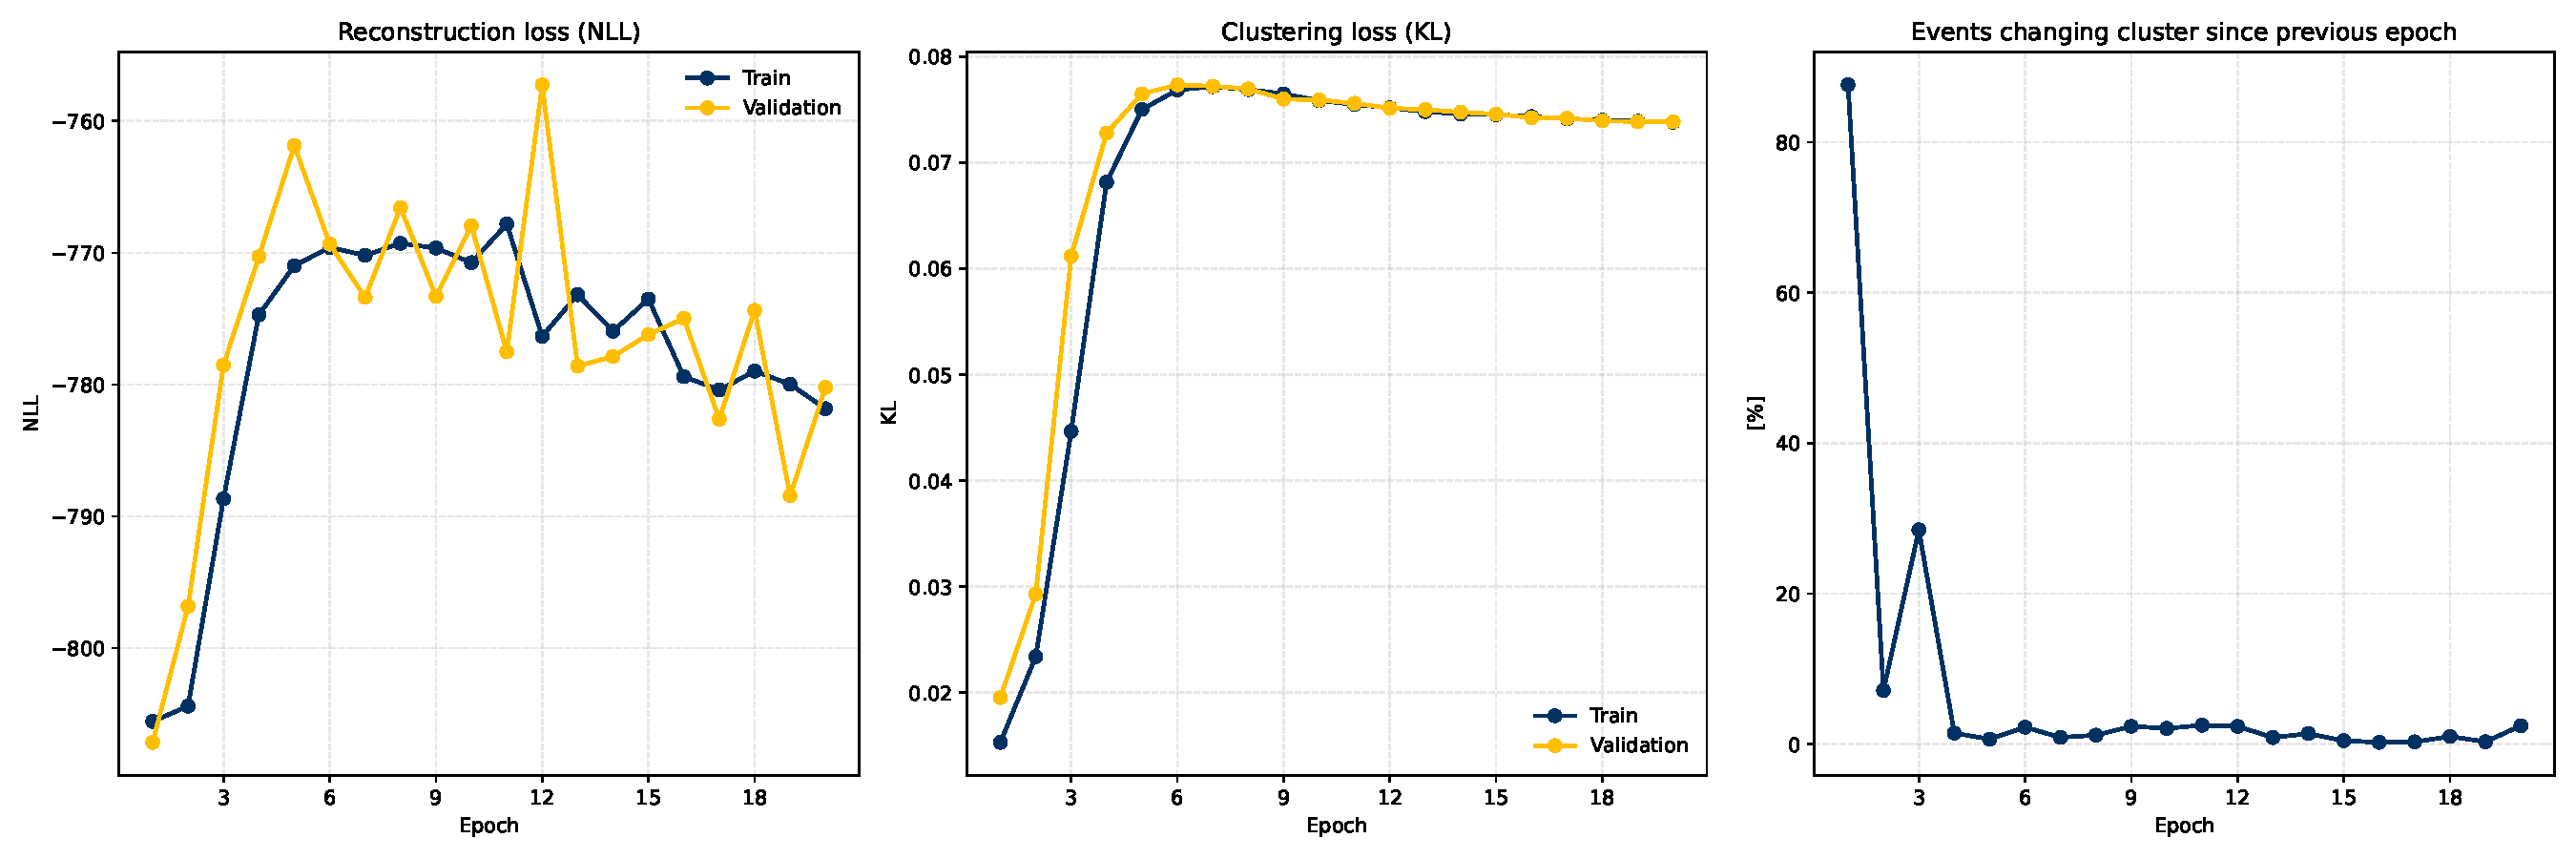
\includegraphics[width=\textwidth]{plots/DTC/clusters_scan/scan_eucl_3cl_training_history.pdf}
    \caption{Training reconstruction and training losses for $K=3$ with Euclidean Distance metric (V08682A).}
    \label{fig:scan-reconstruction_and_losses-K3}
\end{figure}

\begin{figure}[H]
    \centering
    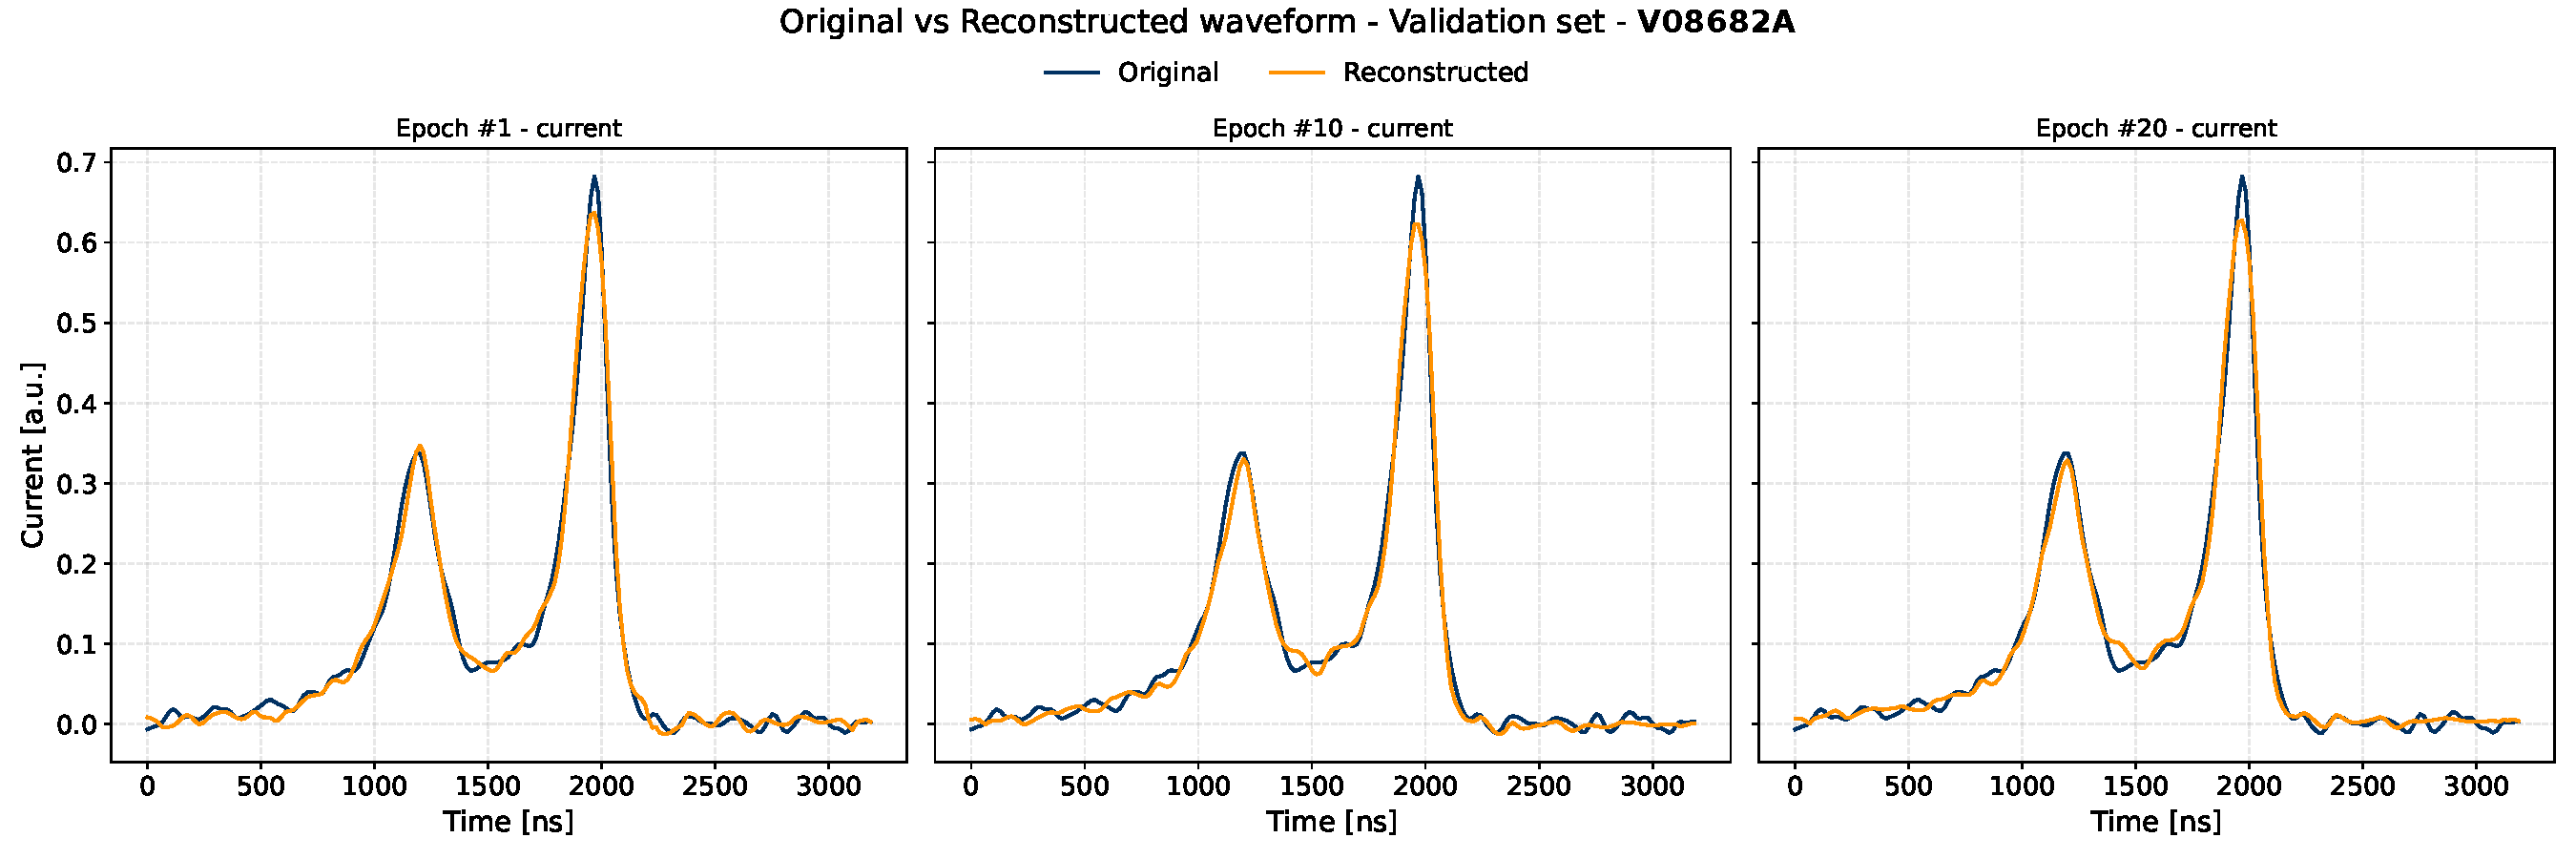
\includegraphics[width=\textwidth]{plots/DTC/clusters_scan/scan_eucl_4cl_training_reconstruction.pdf}
    \par\medskip
    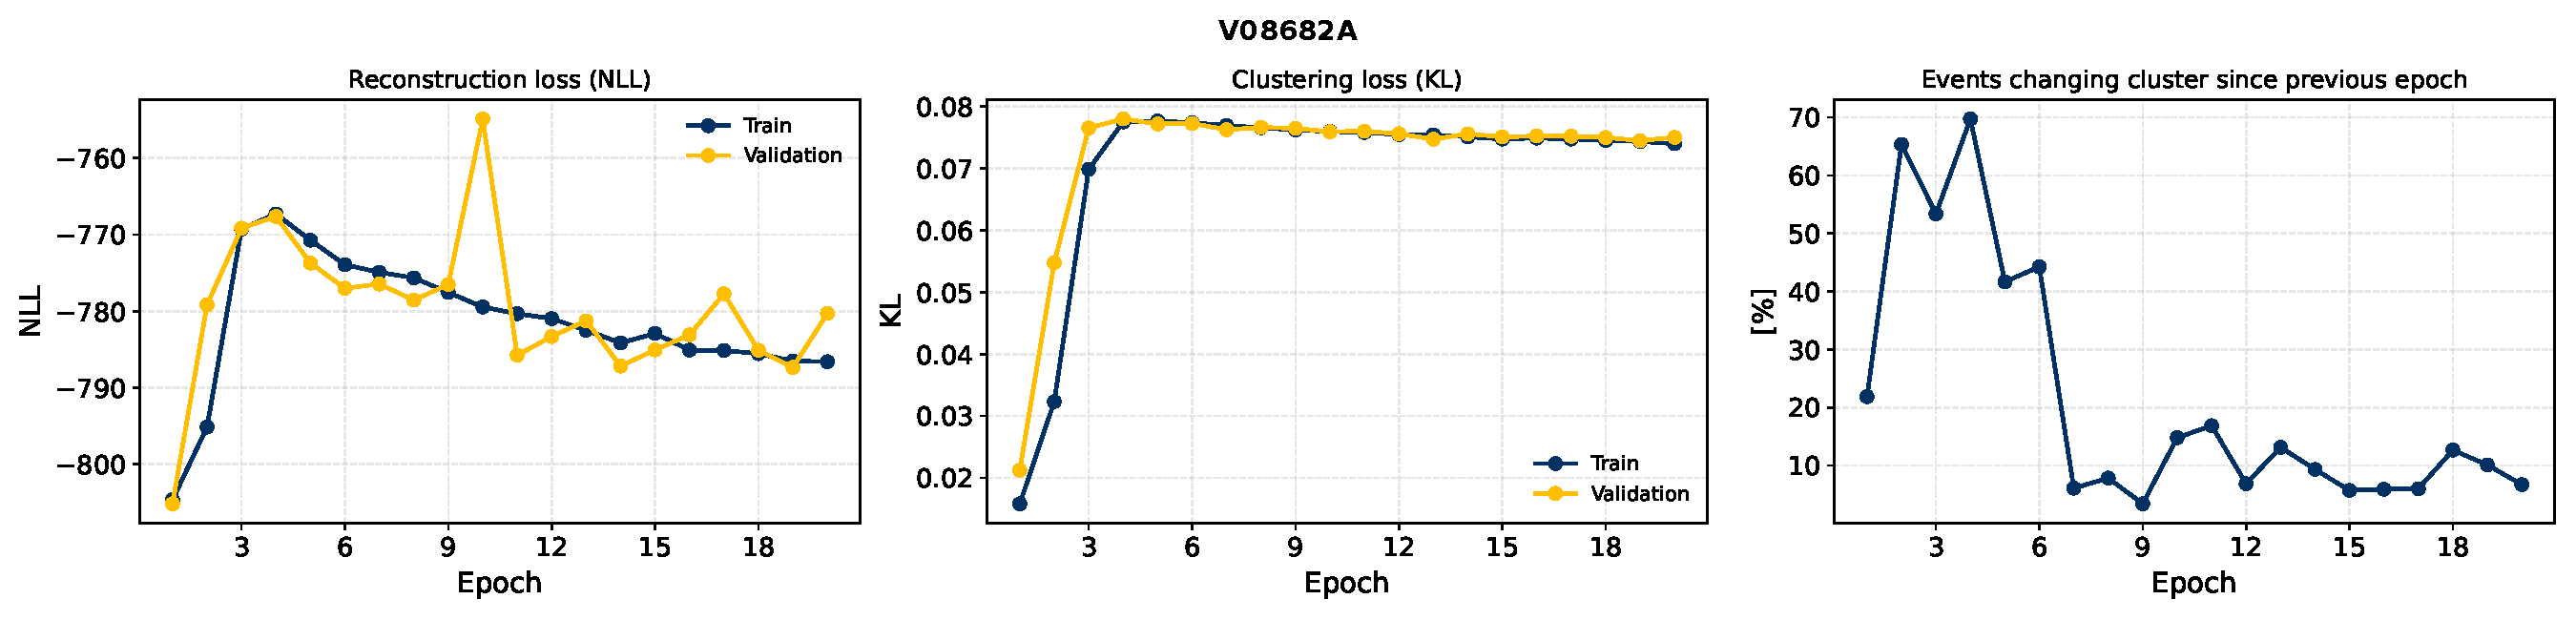
\includegraphics[width=\textwidth]{plots/DTC/clusters_scan/scan_eucl_4cl_training_history.pdf}
    \caption{Training reconstruction and training losses for $K=4$ with Euclidean Distance metric (V08682A).}
    \label{fig:scan-reconstruction_and_losses-K4}
\end{figure}

%=====================================================================
\section{V08682B}
\label{app:DTC-scans-B}
%=====================================================================

\subsection{\texorpdfstring{$\bm{\gamma}$}{gamma} scan results}
Figures \ref{fig:scan-reconstruction_and_losses-gamma10-B}, \ref{fig:scan-reconstruction_and_losses-gamma100-B}, \ref{fig:scan-reconstruction_and_losses-gamma1000-B} and \ref{fig:scan-reconstruction_and_losses-gamma10000-B} show the reconstruction ability and the losses trend for $\gamma= 10, 100, 1000$ and $10000$ respectively for detector V08682B.

% TODO: commento sui risultati dello scan in gamma per V08682B

\begin{figure}[H]
    \centering
    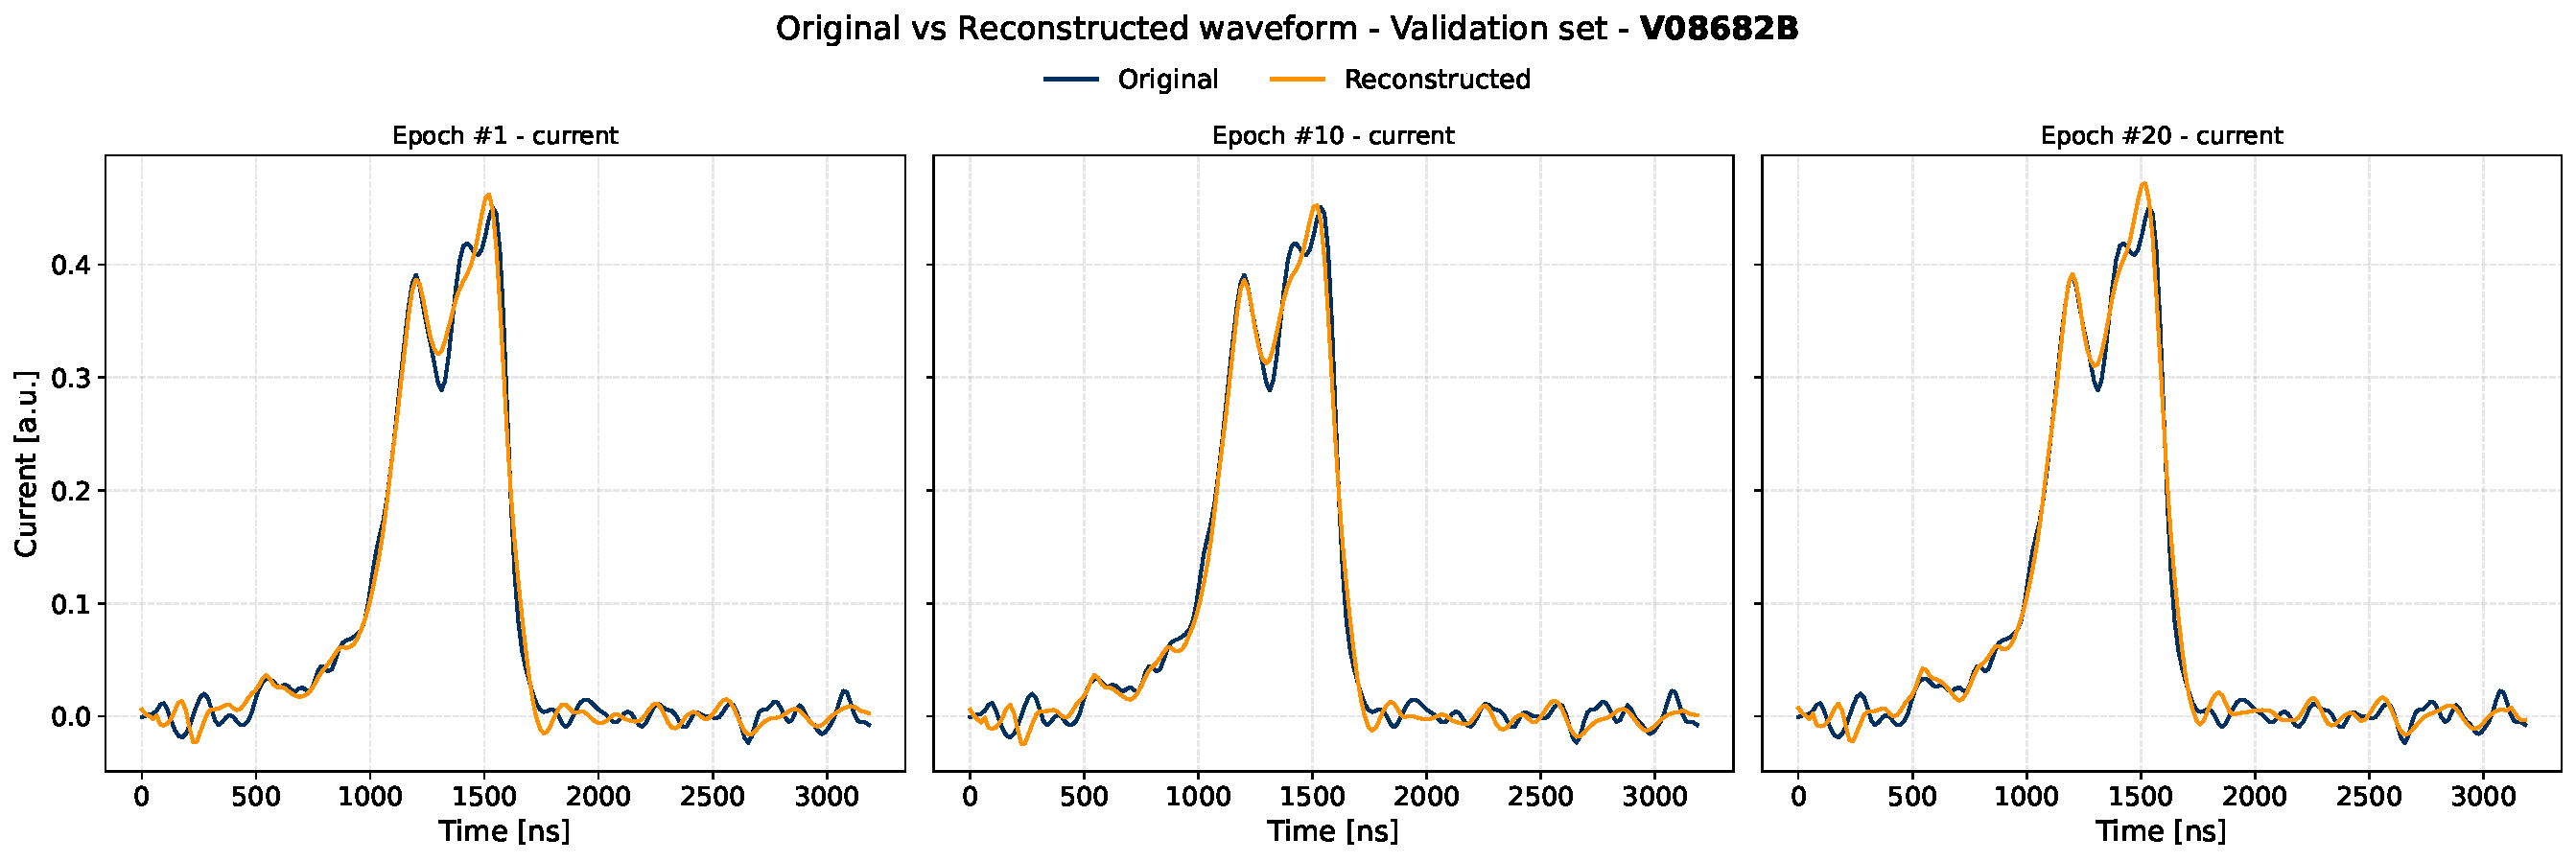
\includegraphics[width=\textwidth]{plots/V08682B/DTC/scan_eucl_gamma10_2cl_training_reconstruction.pdf}
    \par\medskip
    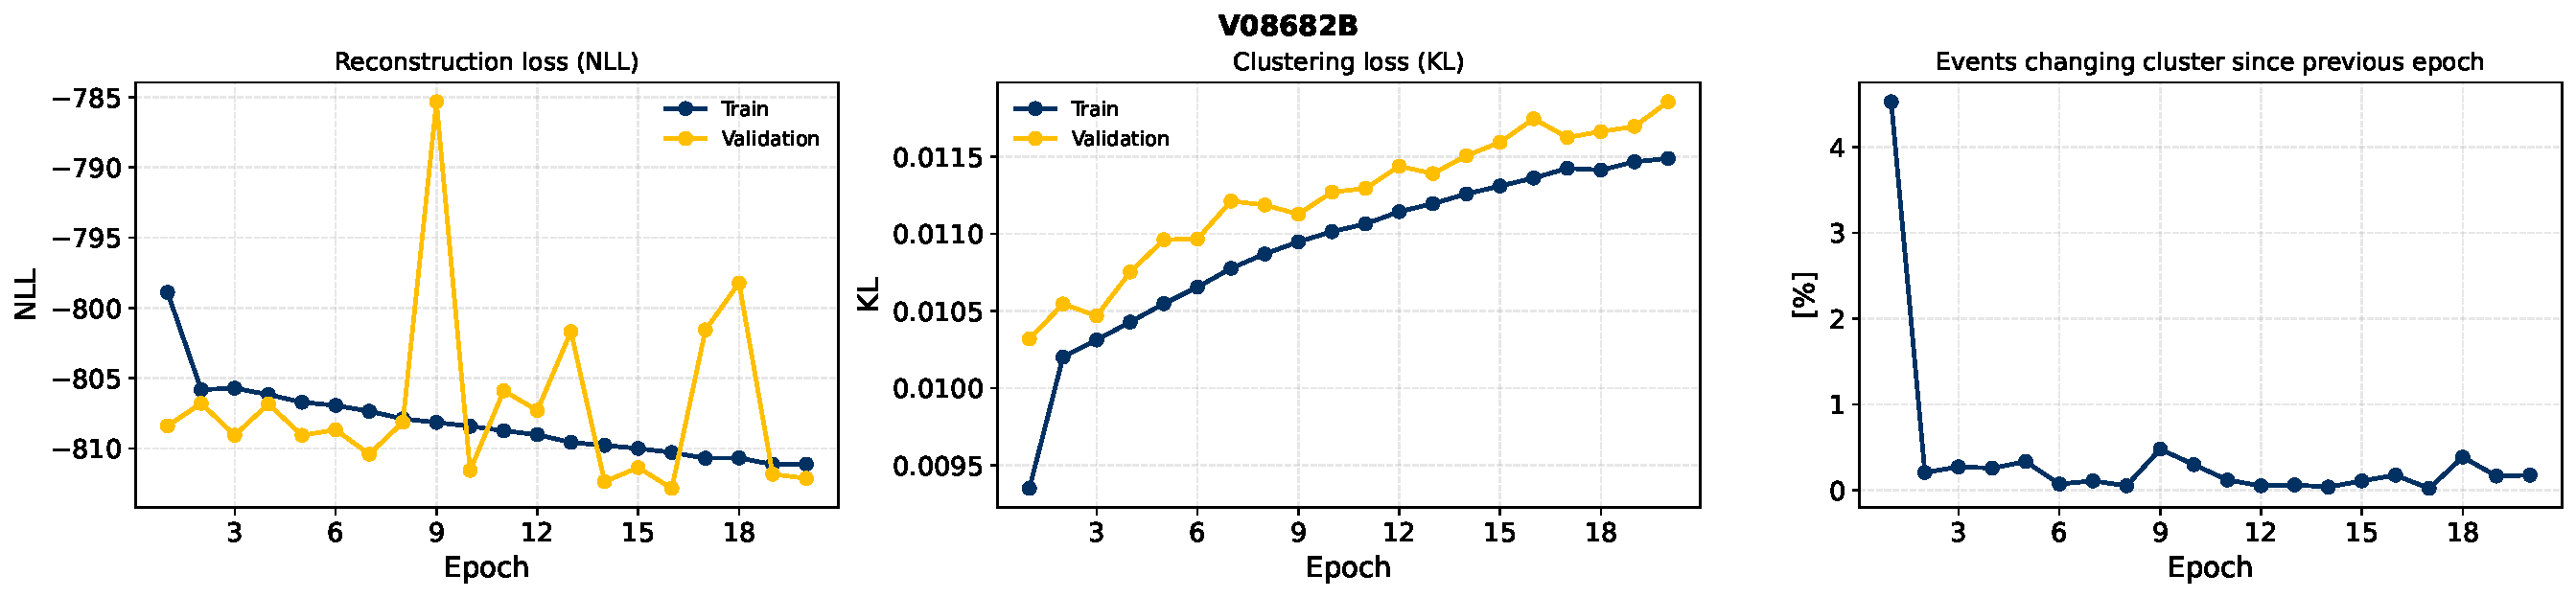
\includegraphics[width=\textwidth]{plots/V08682B/DTC/scan_eucl_gamma10_2cl_training_history.pdf}
    \caption{Training reconstruction and training losses for $\gamma=10$ with Euclidean Distance metric (V08682B).}
    \label{fig:scan-reconstruction_and_losses-gamma10-B}
\end{figure}

\begin{figure}[H]
    \centering
    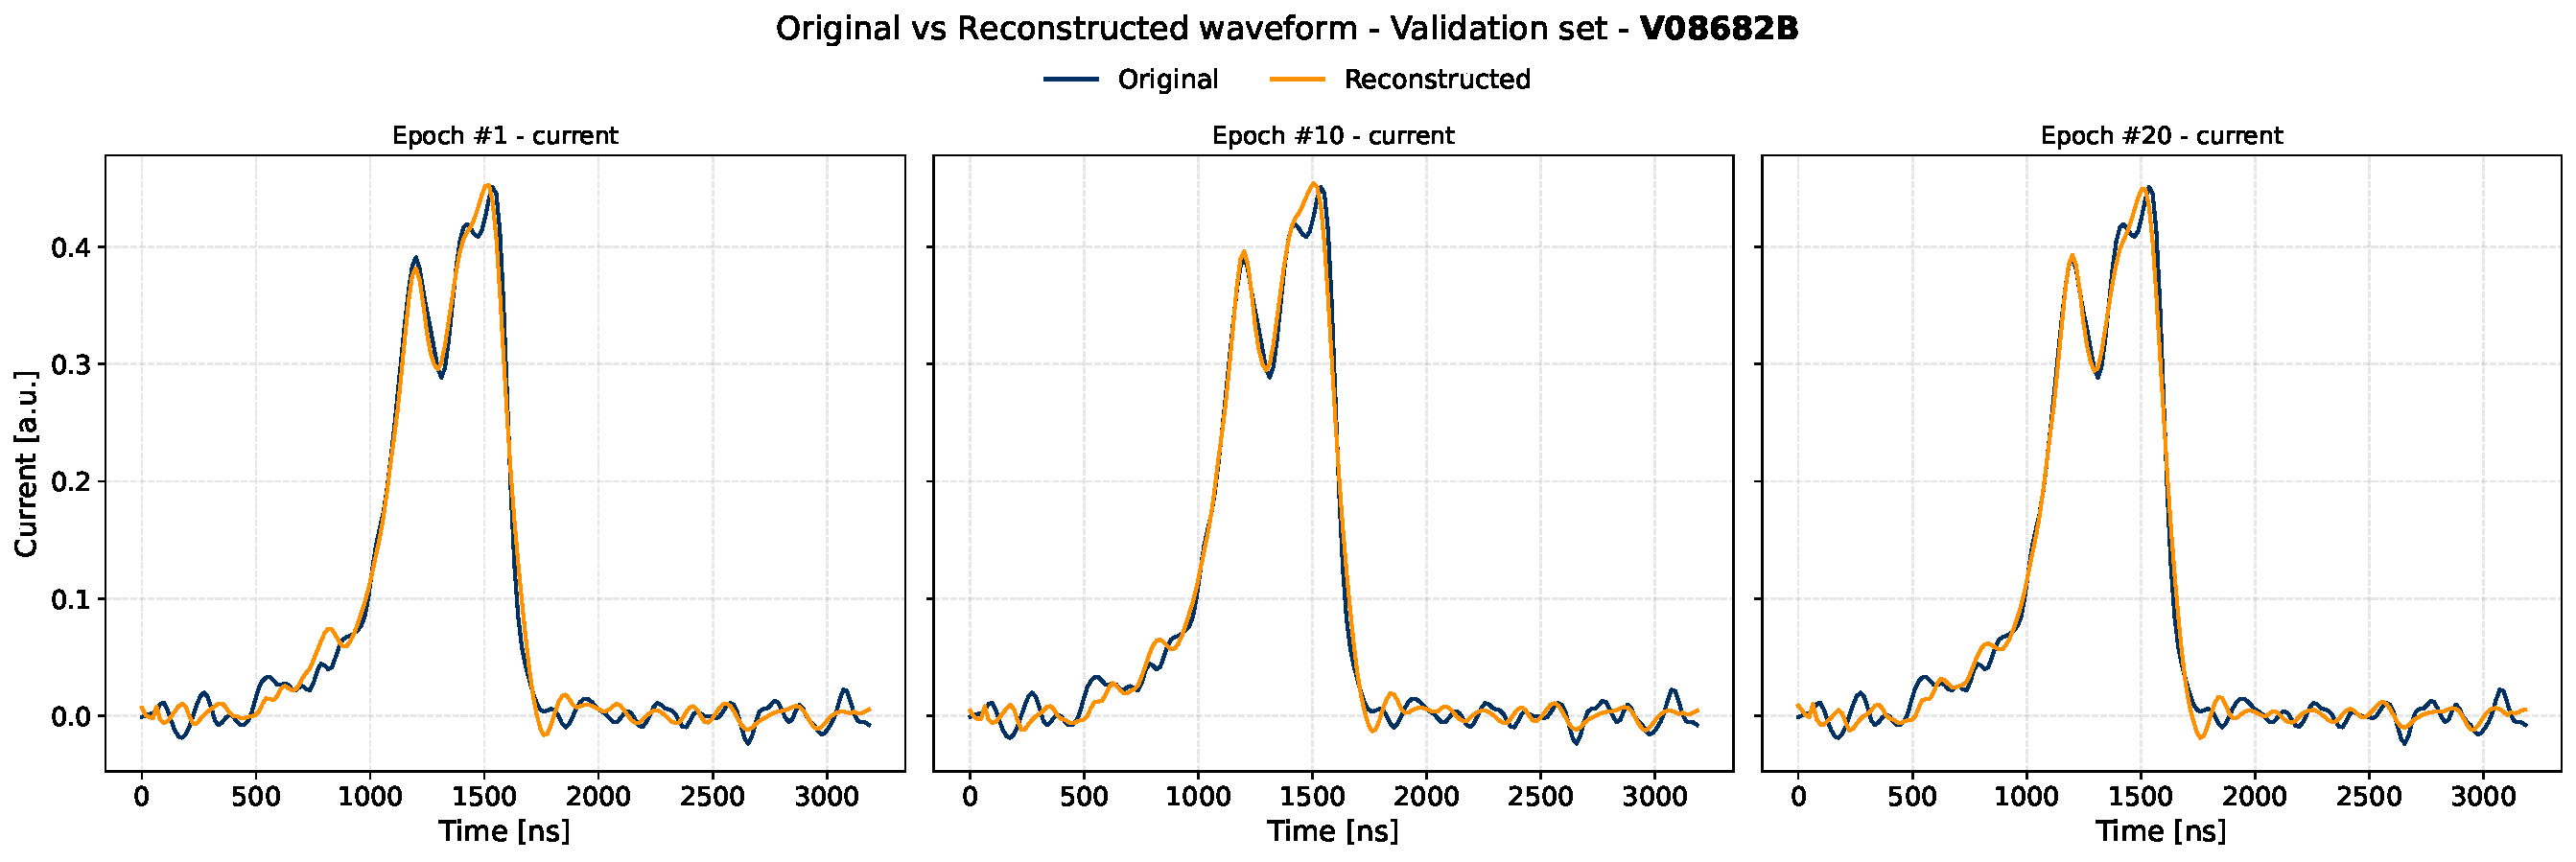
\includegraphics[width=\textwidth]{plots/V08682B/DTC/scan_eucl_gamma100_2cl_training_reconstruction.pdf}
    \par\medskip
    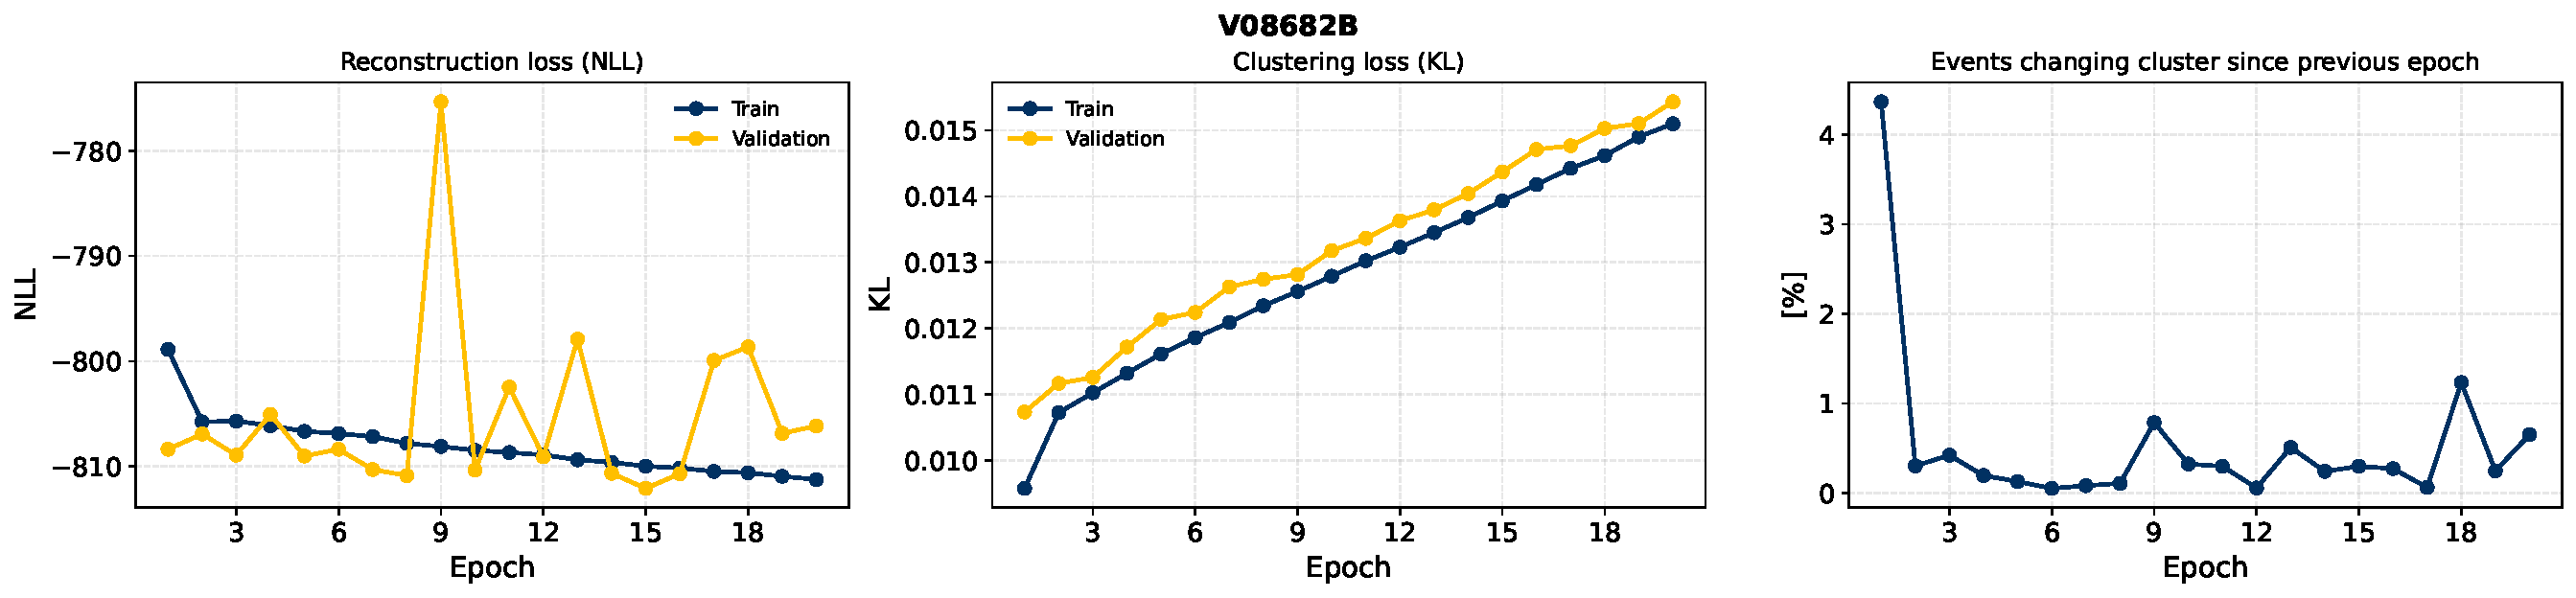
\includegraphics[width=\textwidth]{plots/V08682B/DTC/scan_eucl_gamma100_2cl_training_history.pdf}
    \caption{Training reconstruction and training losses for $\gamma=100$ with Euclidean Distance metric (V08682B).}
    \label{fig:scan-reconstruction_and_losses-gamma100-B}
\end{figure}

\begin{figure}[H]
    \centering
    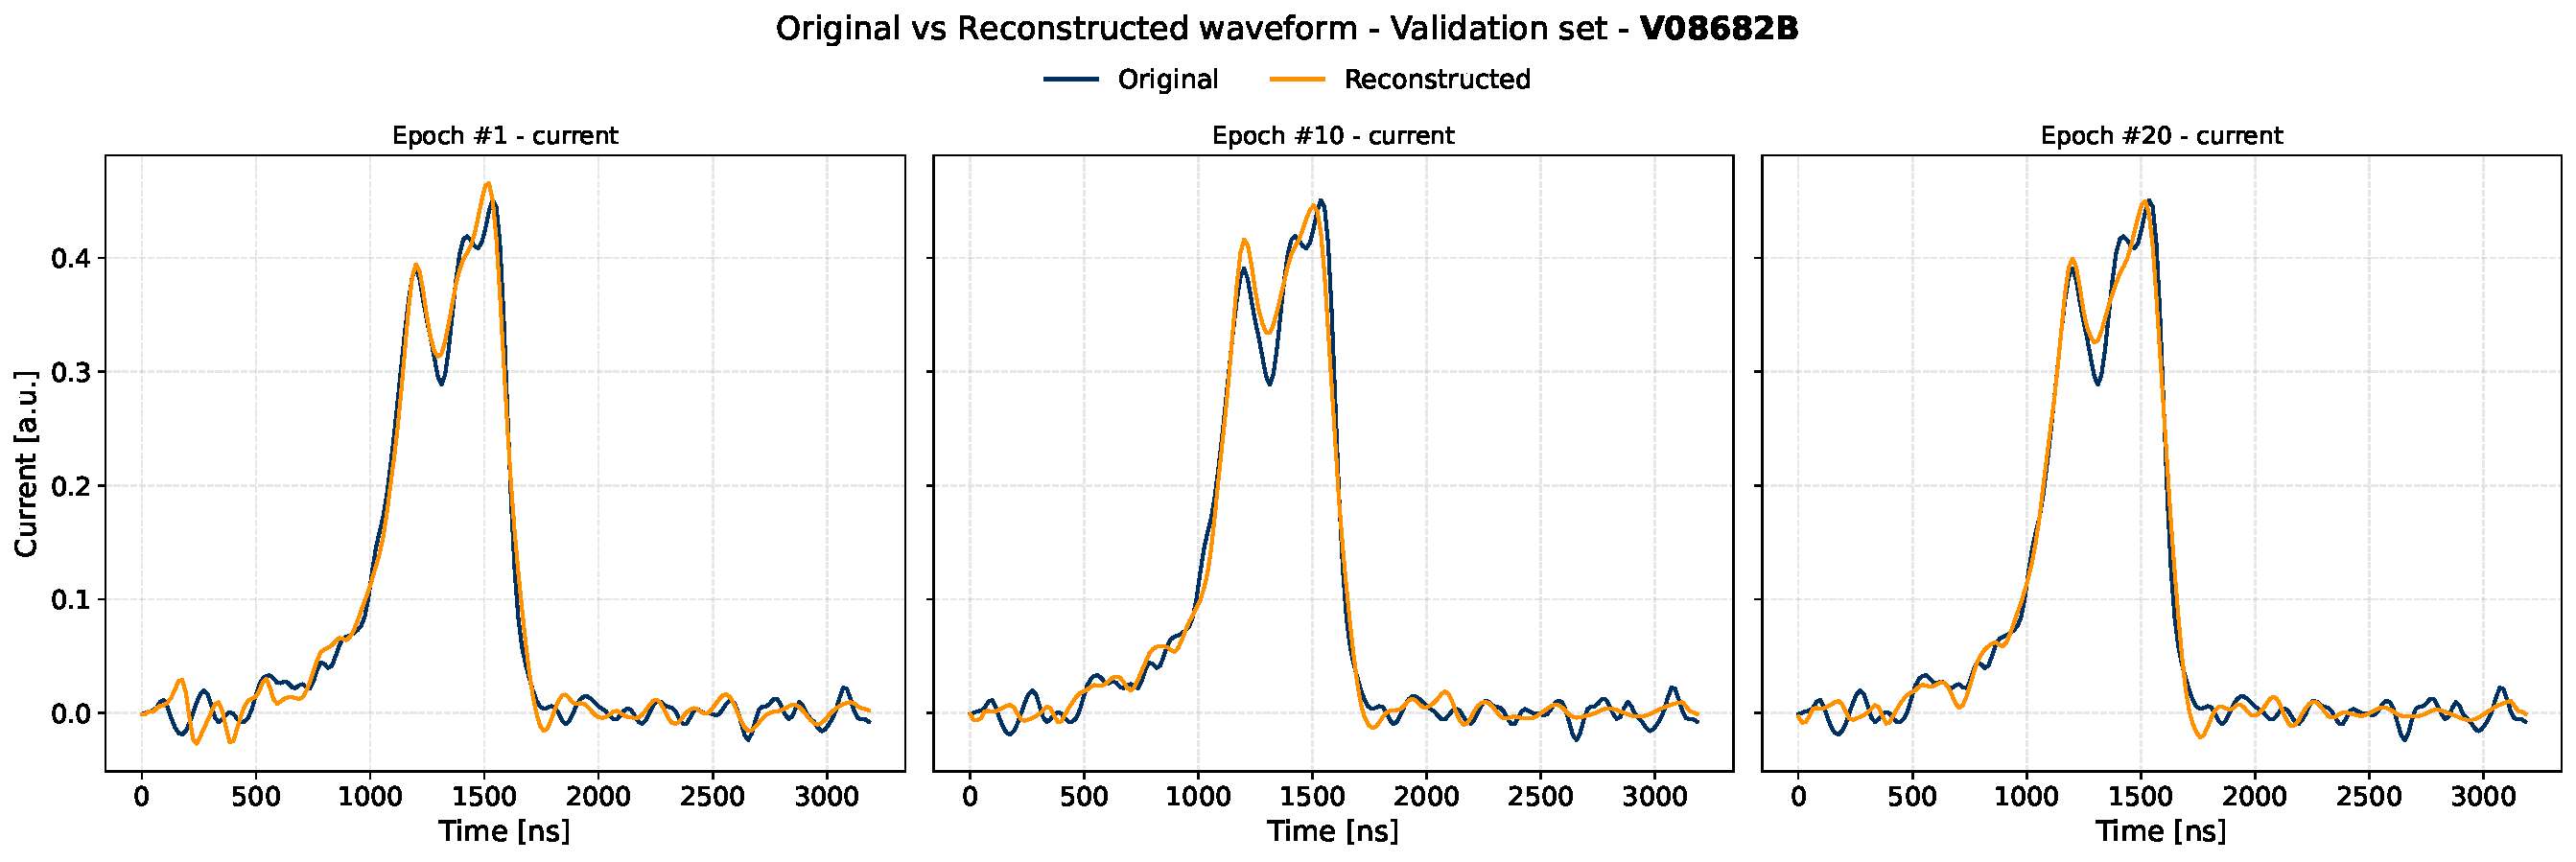
\includegraphics[width=\textwidth]{plots/V08682B/DTC/scan_eucl_gamma1000_2cl_training_reconstruction.pdf}
    \par\medskip
    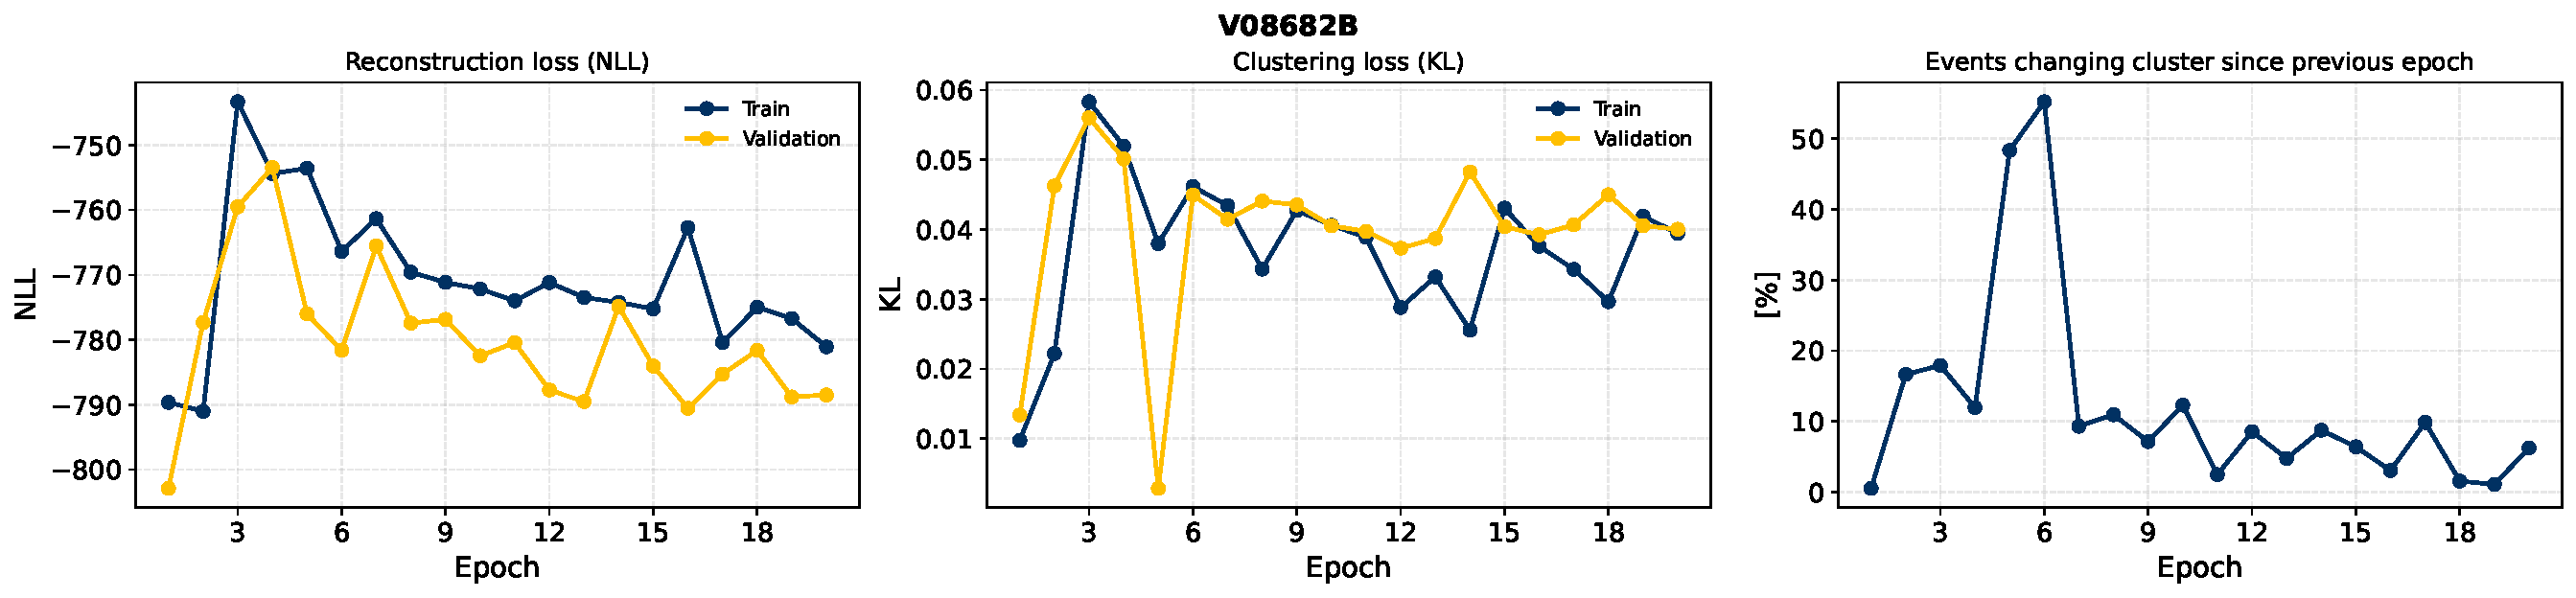
\includegraphics[width=\textwidth]{plots/V08682B/DTC/scan_eucl_gamma1000_2cl_training_history.pdf}
    \caption{Training reconstruction and training losses for $\gamma=1000$ with Euclidean Distance metric (V08682B).}
    \label{fig:scan-reconstruction_and_losses-gamma1000-B}
\end{figure}

\begin{figure}[H]
    \centering
    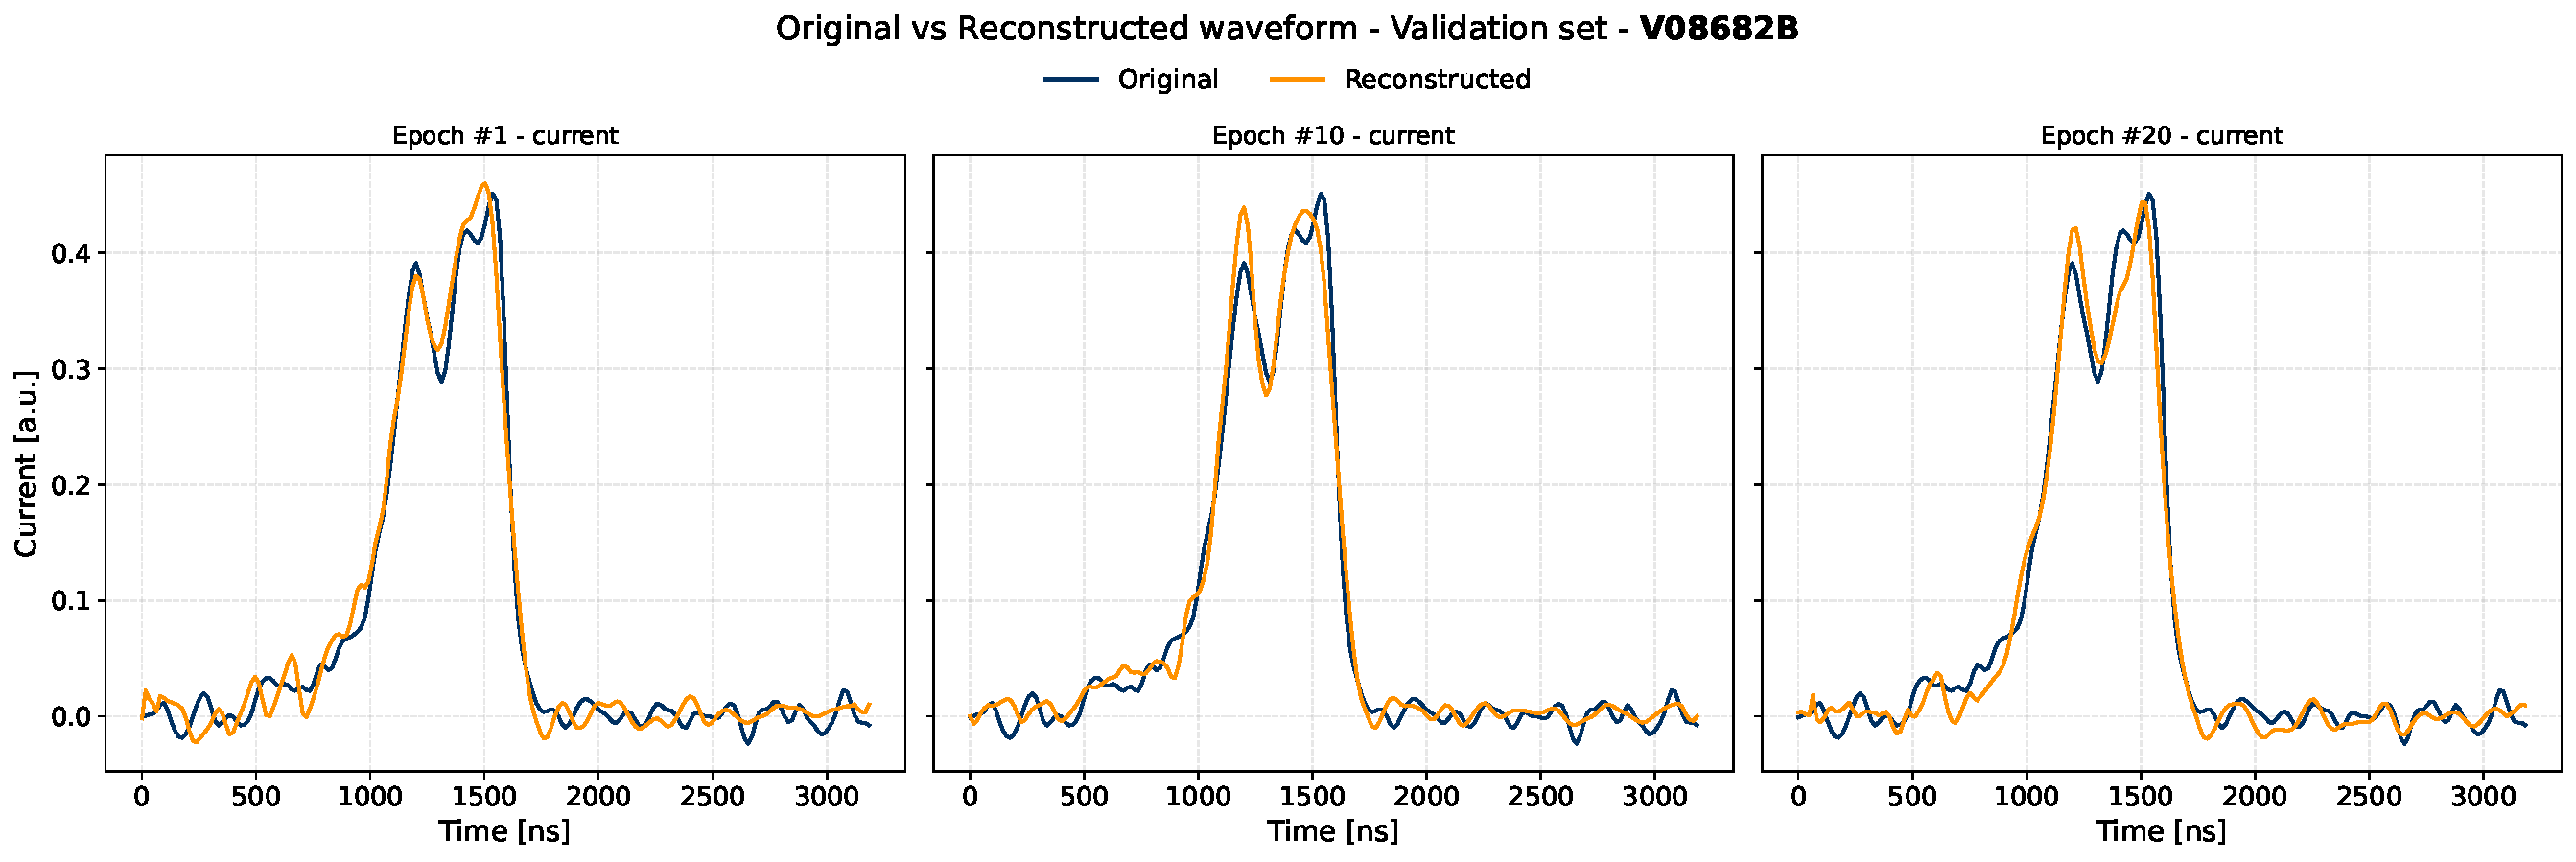
\includegraphics[width=\textwidth]{plots/V08682B/DTC/scan_eucl_gamma10000_2cl_training_reconstruction.pdf}
    \par\medskip
    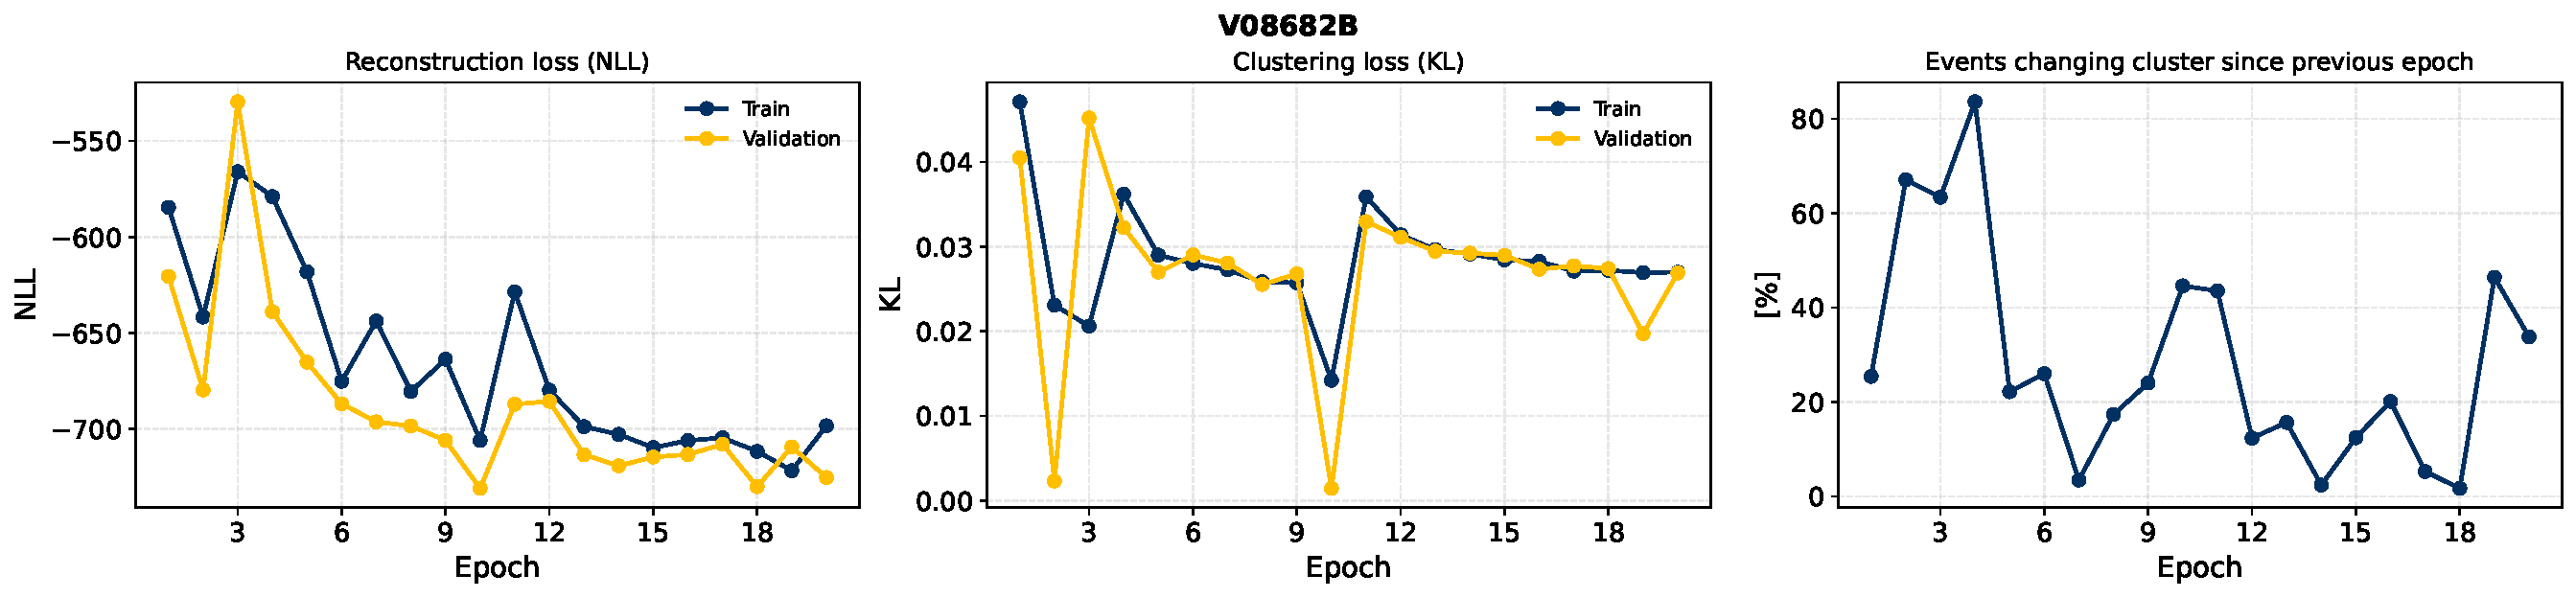
\includegraphics[width=\textwidth]{plots/V08682B/DTC/scan_eucl_gamma10000_2cl_training_history.pdf}
    \caption{Training reconstruction and training losses for $\gamma=10000$ with Euclidean Distance metric (V08682B).}
    \label{fig:scan-reconstruction_and_losses-gamma10000-B}
\end{figure}

\subsection{Clusters scan results}
Figures \ref{fig:scan-reconstruction_and_losses-K3-B} and \ref{fig:scan-reconstruction_and_losses-K4-B} show the reconstruction ability and the losses trend for $K= 3$ and $4$ respectively for detector V08682B. As for V08682A, the $K=2$ configuration is not reported here since it is precisely the one of Fig. \ref{fig:scan-reconstruction_and_losses-gamma1000-B} of the previous Subsection.

\begin{figure}[H]
    \centering
    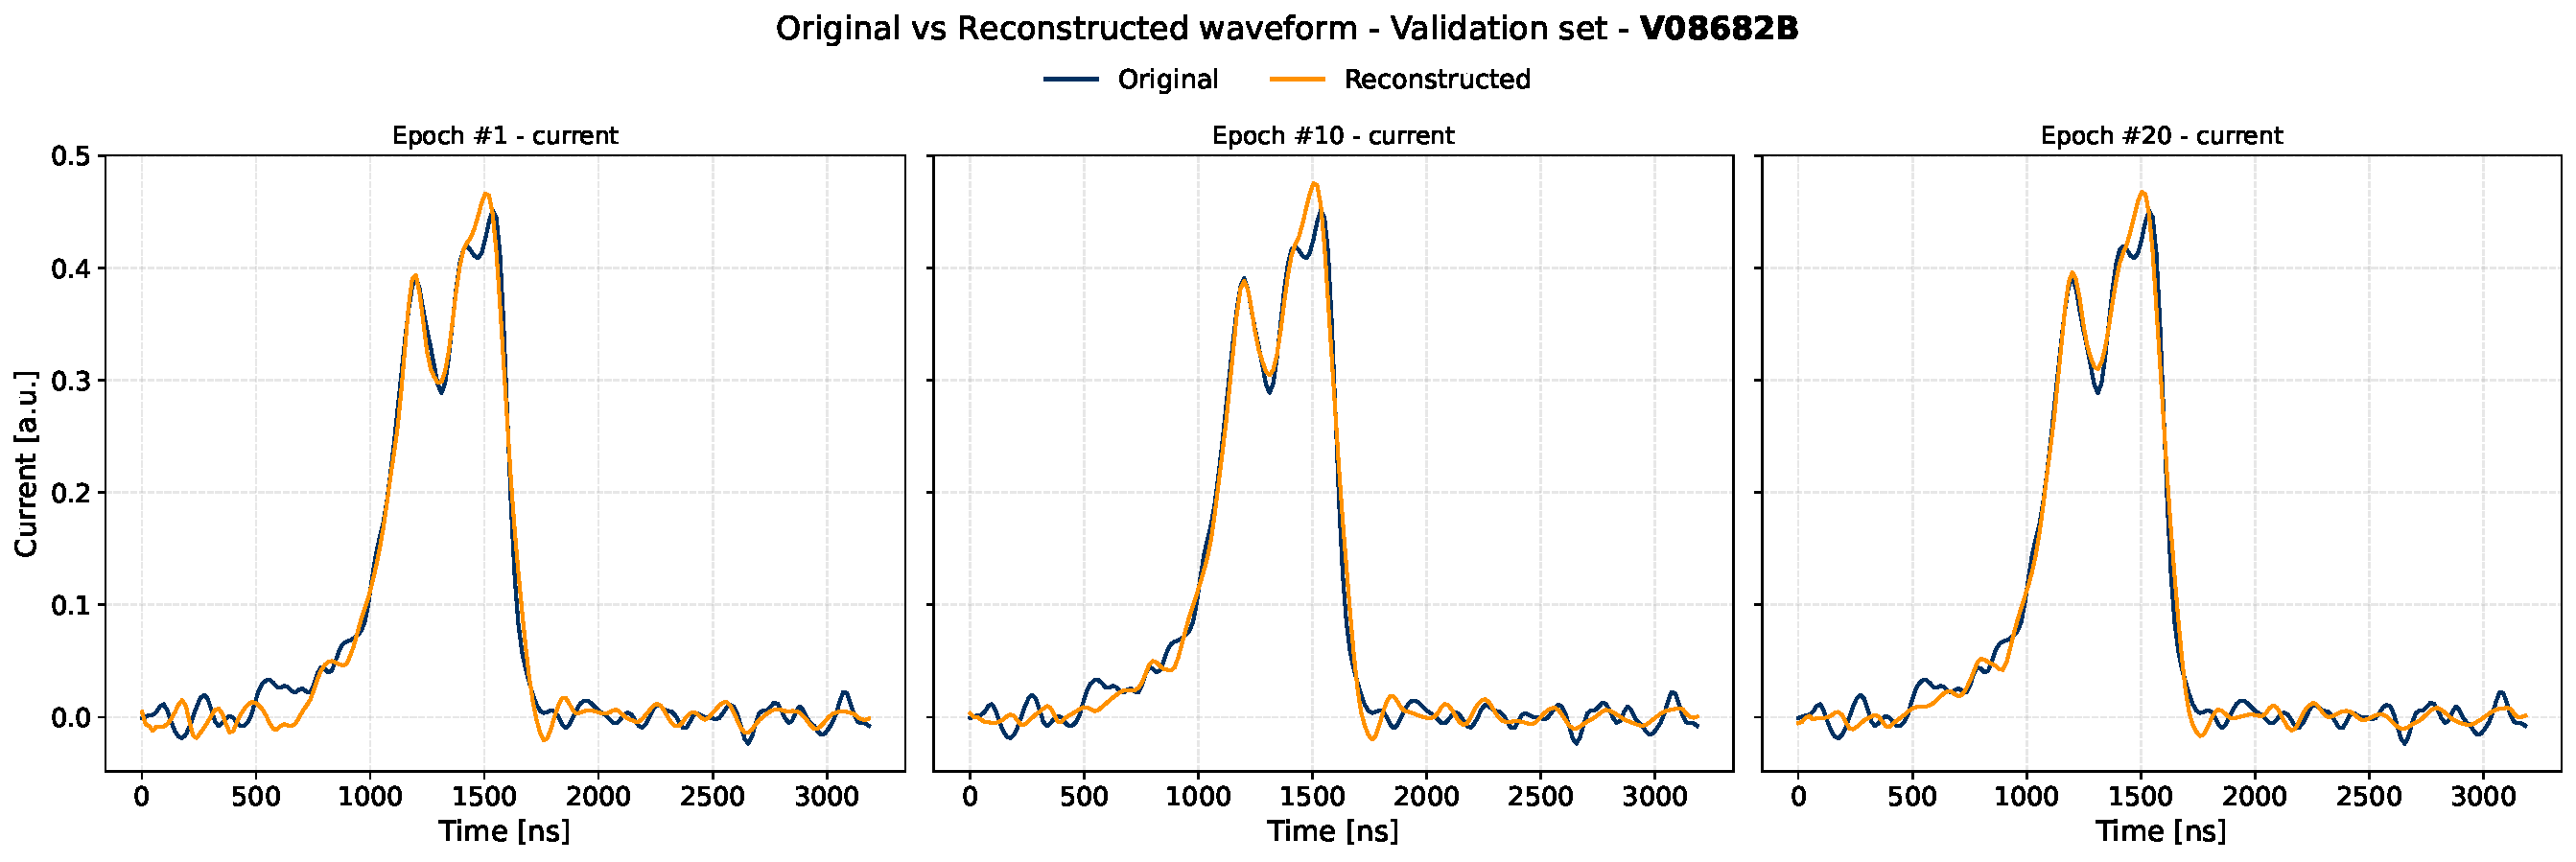
\includegraphics[width=\textwidth]{plots/V08682B/DTC/scan_eucl_3cl_training_reconstruction.pdf}
    \par\medskip
    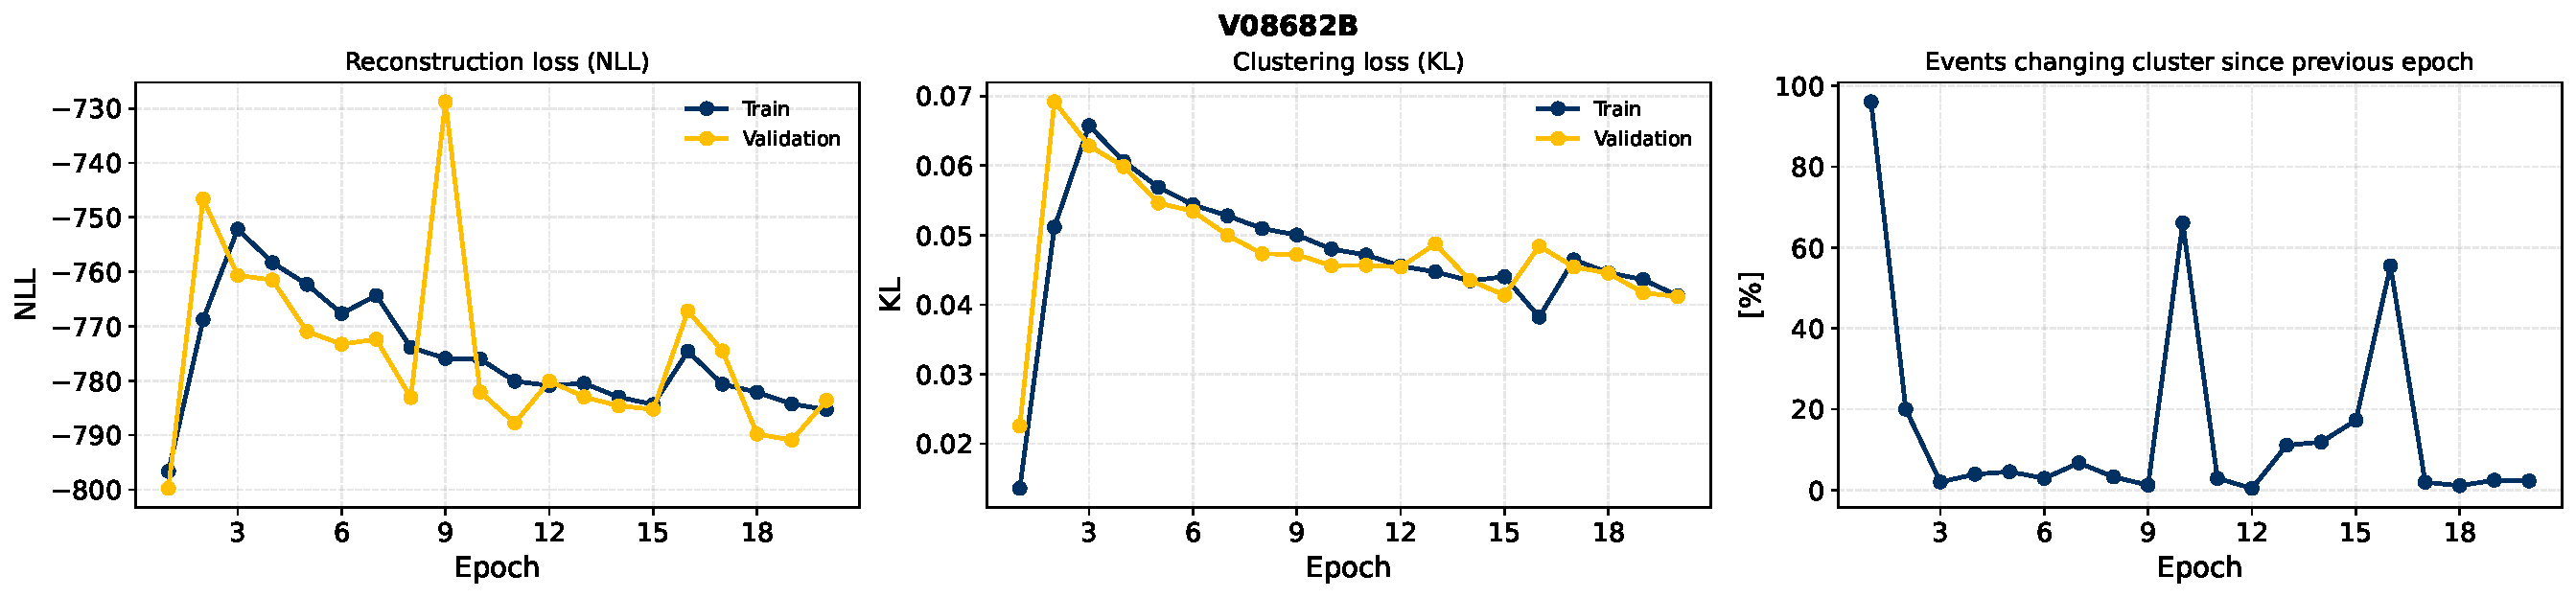
\includegraphics[width=\textwidth]{plots/V08682B/DTC/scan_eucl_3cl_training_history.pdf}
    \caption{Training reconstruction and training losses for $K=3$ with Euclidean Distance metric (V08682B).}
    \label{fig:scan-reconstruction_and_losses-K3-B}
\end{figure}

\begin{figure}[H]
    \centering
    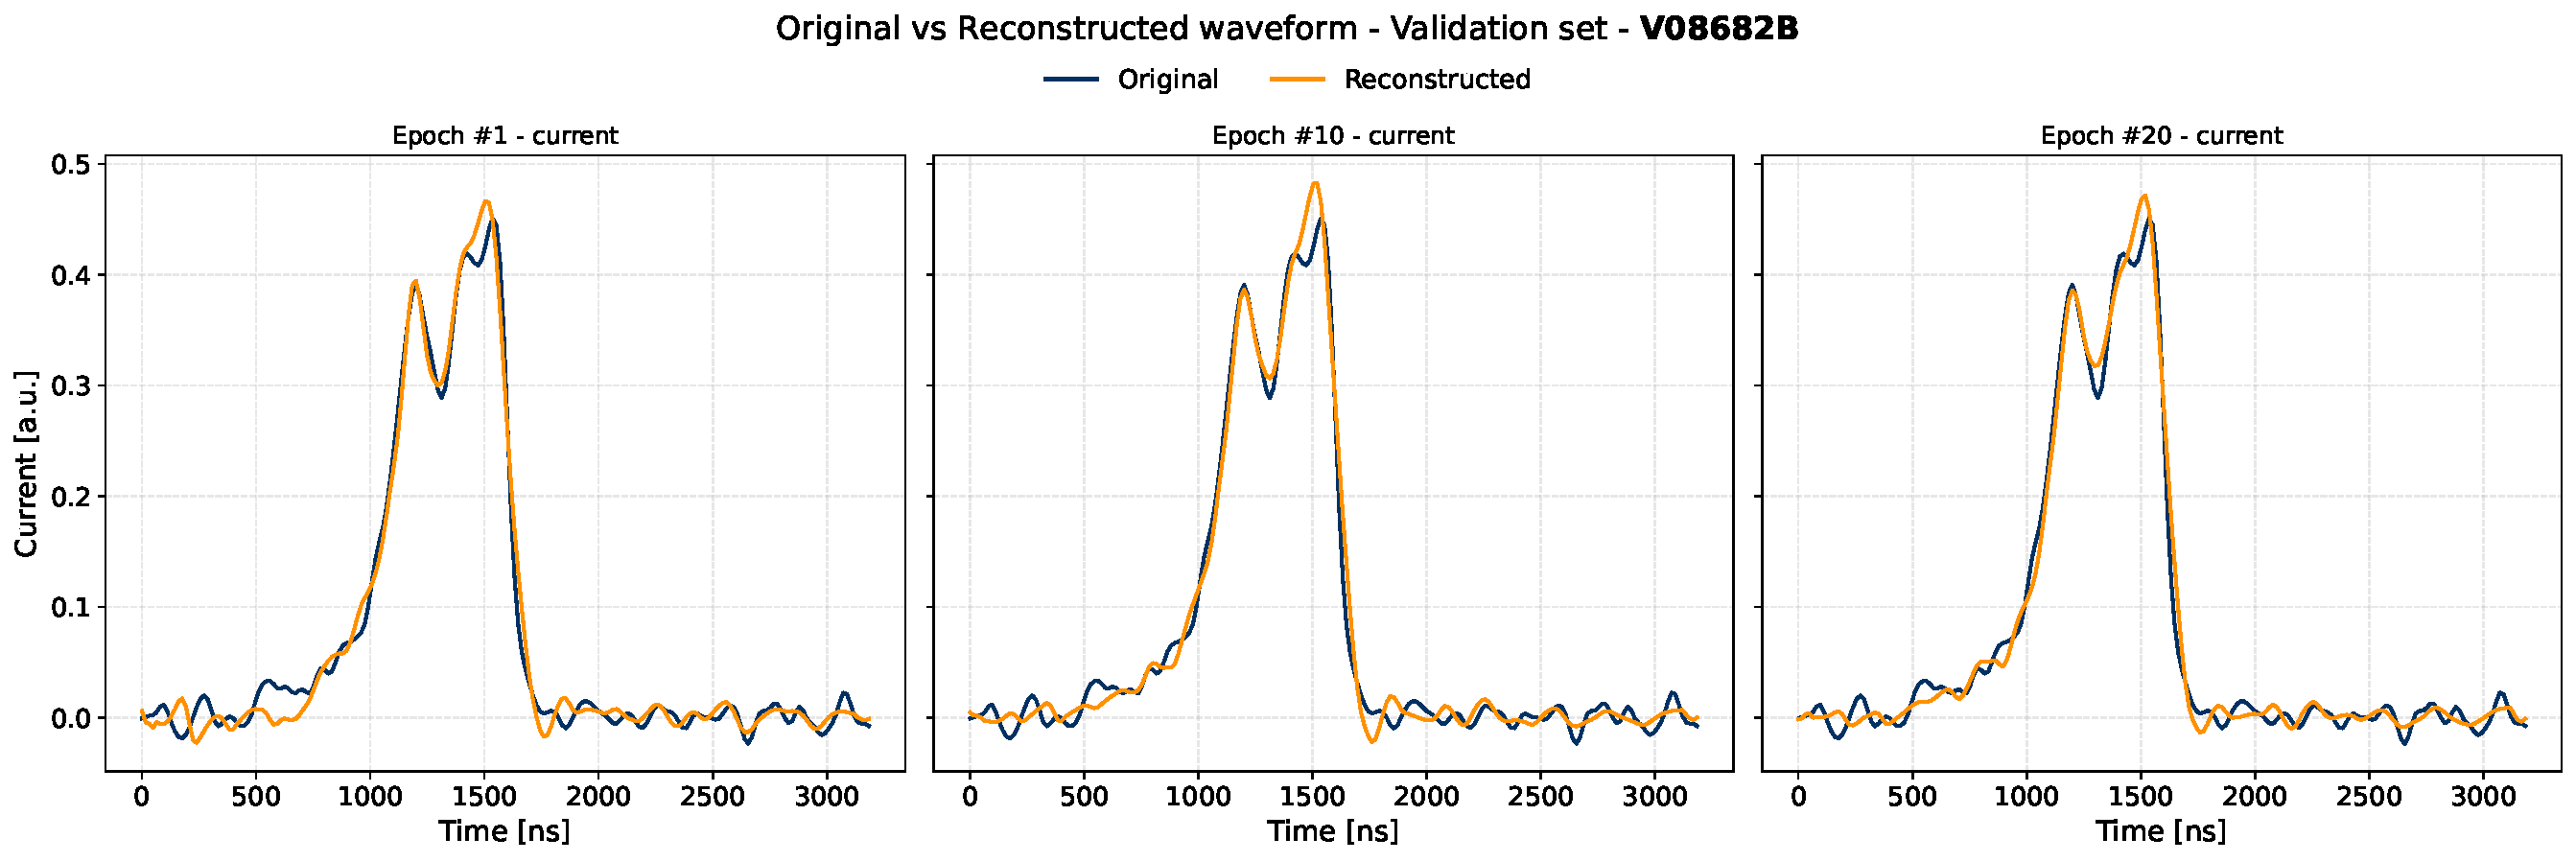
\includegraphics[width=\textwidth]{plots/V08682B/DTC/scan_eucl_4cl_training_reconstruction.pdf}
    \par\medskip
    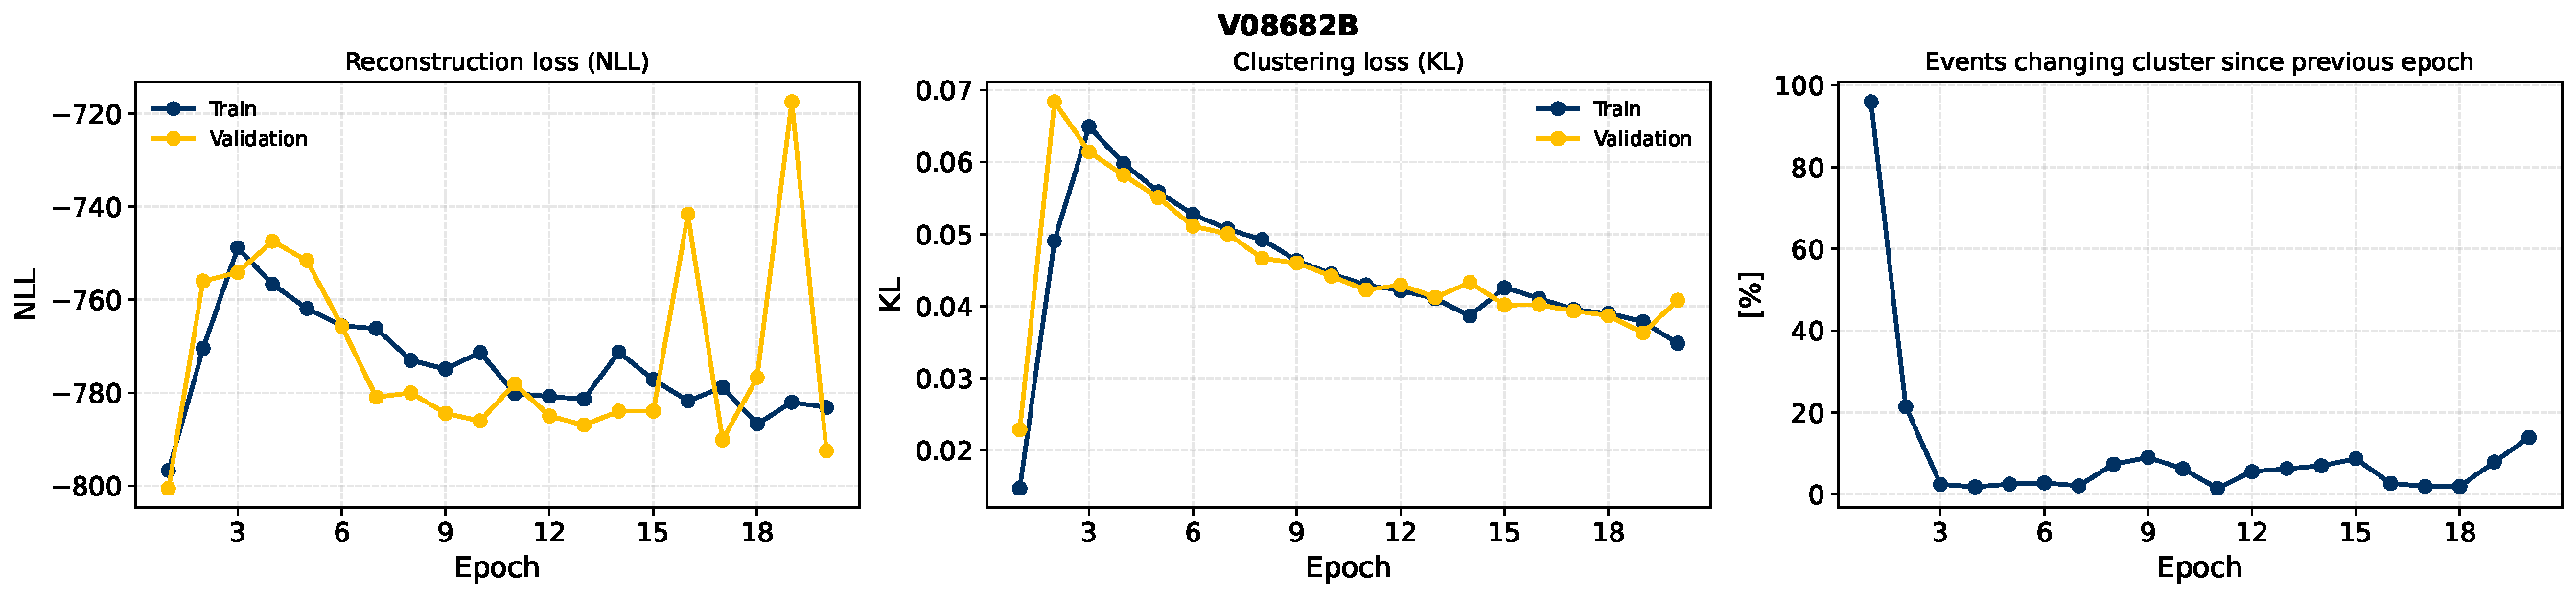
\includegraphics[width=\textwidth]{plots/V08682B/DTC/scan_eucl_4cl_training_history.pdf}
    \caption{Training reconstruction and training losses for $K=4$ with Euclidean Distance metric (V08682B).}
    \label{fig:scan-reconstruction_and_losses-K4-B}
\end{figure}